\documentclass[preprint,12pt]{elsarticle}

% ================= PACKAGES =================
\usepackage[utf8]{inputenc}
\usepackage[T1]{fontenc}
\usepackage{graphicx}
\usepackage{amsmath,amssymb}
\usepackage{booktabs}
\usepackage{multirow}
\usepackage{subcaption}
\usepackage{tikz}
\usetikzlibrary{shapes,arrows,positioning}
\usepackage[numbers,sort&compress]{natbib}
\usepackage{hyperref}
\hypersetup{colorlinks=true,linkcolor=blue,citecolor=blue,urlcolor=blue}
\usepackage{xcolor}
\definecolor{codegray}{rgb}{0.5,0.5,0.5}
\usepackage{listings}
\lstdefinestyle{mystyle}{
    basicstyle=\ttfamily\footnotesize,
    breaklines=true,
    numbers=left,
    numbersep=5pt,
    numberstyle=\tiny\color{codegray},
    frame=single
}
\lstset{style=mystyle}

\newcommand{\rqanswer}[2]{\par\noindent\colorbox{gray!12}{\parbox{0.965\linewidth}{\vspace{0.15cm}\textbf{Answer to #1:} #2\vspace{0.15cm}}}\par\vspace{0.25cm}}

\journal{Journal of Systems and Software}

% ================= DOCUMENT =================
\begin{document}

\begin{frontmatter}

\title{Chain-of-Thought Fine-Tuning and Retrieval-Augmented Generation for LLM-Based Vulnerability Detection in Low-Resource Smart Contract Languages: A Study on Algorand and Solana}

%% NOTE FOR AUTHORS: adjust author order, affiliations, and corresponding-author
%% designation as appropriate before submission. Populated from the source thesis
%% front matter (Universit\`a degli Studi di Salerno, Dipartimento di Informatica).
\author[unisa]{Nicola Tortora}
\author[unisa]{Biagio Boi\corref{cor1}}
\ead{biagioboi@gmail.com}
\author[unisa]{Christiancarmine Esposito}

\cortext[cor1]{Corresponding author.}
\affiliation[unisa]{organization={Department of Computer Science, University of Salerno},
            city={Fisciano},
            postcode={84084},
            state={SA},
            country={Italy}}

\begin{abstract}
Smart contracts written for low-resource blockchain ecosystems -- Algorand's PyTeal and Solana's Rust -- are poorly served by mainstream static-analysis tooling, which targets EVM-based chains, and are underrepresented in LLM pre-training corpora. Applied zero-shot to these languages, LLMs latch onto superficial syntactic correlations rather than a vulnerability's causal logic, producing hallucinated findings and missed detections. This paper proposes and evaluates a hybrid, LLM-centric vulnerability-detection pipeline combining (i) supervised fine-tuning on a curated Chain-of-Thought corpus that teaches a medium-scale open-weight model (Qwen3-32B) a step-by-step audit process, and (ii) Retrieval-Augmented Generation (RAG) that injects, at inference time, semantically matched vulnerable code snippets and security checklists from a vector knowledge base of LLM-generated contract descriptions. The pipeline is evaluated independently on both ecosystems to test whether it generalizes beyond a single low-resource language. All results are averaged over 5 independently seeded stochastic samples per configuration, reported as mean $\pm$ standard deviation. On 45 held-out Algorand contracts (eight vulnerability classes), fine-tuning with RAG raises F1 from 0.45$\pm$0.08 to 0.80$\pm$0.04 (Qwen3-32B) and up to 0.81$\pm$0.01 (QwQ-32B), with fine-tuning driving most of the precision gain and RAG most of the recall gain, approaching -- though not matching -- a state-of-the-art generalist model an order of magnitude larger while remaining deployable on-premise. On 97 held-out Solana contracts (seven classes), the same recipe raises F1 from 0.33$\pm$0.03 to 0.57$\pm$0.06, following the same qualitative pattern at lower absolute performance, reflecting Rust's added cross-instruction and cross-program-invocation reasoning burden; part of this gap traces to retrieval knowledge-base coverage rather than model capacity. Manual verification of raw model outputs confirms the gains are genuine, while showing non-fine-tuned models systematically over-report checklist findings -- a precision failure automated first-match parsing under-counts. A dedicated stability analysis further shows that RAG reduces sample-to-sample variance as well as raising the mean, and that scrutinizing an initially implausible resampled result exposed two independent evaluation-pipeline defects, both corrected before the results reported here were produced. These results indicate in-context retrieval alone approaches the accuracy ceiling for large generalist models, while fine-tuning remains necessary for a medium-scale local model to close most, though not all, of that gap -- relevant to data-sovereignty-constrained, on-premise deployments, and consistent across two structurally different smart-contract languages. Code, prompts, and both Chain-of-Thought datasets are released for reproducibility.
\end{abstract}

\begin{keyword}
Smart contract security \sep Algorand \sep PyTeal \sep Solana \sep Rust \sep Large language models \sep Retrieval-augmented generation \sep Parameter-efficient fine-tuning \sep Vulnerability detection \sep Chain-of-thought reasoning
\end{keyword}

\end{frontmatter}

%% ---------------------------------------------------------------
%% HIGHLIGHTS (submit separately as a .docx/.tex per journal
%% instructions; reproduced here for completeness). Max ~85
%% characters per bullet, 3-5 bullets.
%% ---------------------------------------------------------------
% \begin{itemize}
%   \item An LLM-centric hybrid pipeline is proposed for PyTeal vulnerability audit.
%   \item CoT fine-tuning teaches 32B open models a step-by-step audit procedure.
%   \item A semantic-abstraction RAG module retrieves vulnerability-matched snippets.
%   \item RAG improves F1-score across every tested model scale and training regime.
%   \item Fine-tuned 32B models plus RAG approach the accuracy of a 20x larger LLM.
% \end{itemize}

\section{Introduction}
\label{sec:intro}

Blockchain technology has redefined digital trust by enabling the decentralized execution of programmable agreements, or \emph{smart contracts}, without intermediaries. Among post-Ethereum platforms, Algorand and Solana both pursue high throughput and low latency through consensus and runtime designs quite different from Ethereum's -- Algorand via a Pure Proof-of-Stake (PPoS) protocol with immediate transaction finality, Solana via a Proof-of-History-ordered, parallel-execution (Sealevel) runtime. Neither design relaxes the central security constraint of the smart-contract paradigm: once deployed, contract code is effectively immutable, so any residual vulnerability is permanent and can lead to irreversible financial loss.

Smart contract development on Algorand takes place on the Algorand Virtual Machine (AVM) through \textbf{PyTeal}, a Python \emph{embedded domain-specific language} that compiles to the low-level TEAL bytecode actually executed on-chain; syntactically valid Python can compile into an insecure TEAL program, e.g., because a required authorization check was never encoded. Solana programs, by contrast, are typically written directly in \textbf{Rust} (often with the Anchor framework) and compiled to the SBF (eBPF-derived) bytecode run by the Sealevel runtime. Here the risk is architectural rather than a translation artifact: every account passed into an instruction is an untyped, attacker-suppliable reference, so the program itself is responsible for verifying ownership, signer status, account type, and cross-program-invocation (CPI) targets -- omitting any one of these checks, or failing to canonicalize a program-derived address's bump seed, yields an exploitable vulnerability with no counterpart in account-model chains such as Ethereum. Auditing either stack is challenging, and two dominant approaches currently fall short.

\emph{Static-analysis tools} (e.g., Slither, SmartCheck) are effective at flagging known syntactic patterns but were built for the Ethereum Virtual Machine (EVM); they cannot be ported to Algorand's stack-based execution model or to Solana's account-centric, CPI-driven one, and even where language-specific tooling exists (e.g., early Solana-focused linters), rule-based analysis struggles with vulnerabilities that depend on contract-specific business logic.

\emph{General-purpose LLMs} (e.g., GPT-5, Gemini, DeepSeek) exhibit strong reasoning capabilities on code but degrade sharply on low-resource, domain-specific languages and idioms. PyTeal and TEAL are comparatively rare in public pre-training corpora, unlike Solidity; Rust itself is well represented, but the Solana-specific conventions that determine security -- Anchor account constraints, CPI patterns, PDA derivation -- are a narrow, underrepresented slice of that corpus. In a zero-shot setting, generalist LLMs tend to hallucinate non-existent syntax or overlook platform-specific security primitives -- transaction \emph{rekeying} and \texttt{CloseRemainderTo} on Algorand, unchecked signer/owner fields and non-canonical bump seeds on Solana -- that have no direct analogue on EVM-based chains.

This paper is a substantial extension of our earlier taxonomic study on prompt engineering versus fine-tuning for LLM-based vulnerability detection on Algorand and Solana \citep{boi2025}, which established that PyTeal is markedly harder for LLMs to reason about than Rust and that fine-tuning is necessary to move base models beyond a null F1-score on several vulnerability classes. Building on that finding, we ask two research questions that the earlier study left open:

\begin{itemize}
    \item \textbf{RQ1.} Does supervised Chain-of-Thought fine-tuning remain necessary once inference-time retrieval of vulnerability-specific context is available, or can Retrieval-Augmented Generation alone close the domain gap?
    \item \textbf{RQ2.} Does the answer to RQ1 depend on model scale, i.e., do medium-scale open-weight models (on the order of 32B parameters) and massive generalist models (on the order of $10^{2}$--$10^{3}$B parameters) benefit differently from fine-tuning and retrieval?
\end{itemize}

To answer these questions we design, implement, and evaluate a hybrid, \emph{LLM-centric} vulnerability-detection pipeline, instantiated independently for PyTeal and for Rust, that combines two adaptation strategies. First, for each language we construct a curated instruction-tuning corpus in which every training response is decomposed into an explicit reasoning trace (Chain-of-Thought, CoT) followed by a structured verdict, and use it to fine-tune 32B reasoning-oriented open-weight models (Qwen3-32B for both languages, and additionally QwQ-32B for Algorand) via quantized low-rank adaptation (QLoRA). Second, we implement a RAG module, one knowledge base per language, that retrieves the snippets and security checklists most relevant to the contract under analysis; to avoid conflating functional similarity with security similarity, retrieval is performed over LLM-generated, syntax-agnostic \emph{security descriptions} of contract logic rather than over raw source code. Both components are evaluated in isolation and in combination on each language independently, with the Algorand configuration additionally benchmarked against a state-of-the-art generalist LLM (DeepSeek-V3.2) used purely through in-context learning.

The contributions of this paper are as follows:
\begin{enumerate}
    \item Two reusable vulnerability knowledge bases and dataset-construction methodologies -- eight OWASP-mapped classes for Algorand and seven for Solana -- together with a multi-task instruction-tuning schema (vulnerability detection, targeted vulnerability verification, semantic code description) tailored to a RAG-compatible pipeline.
    \item A Chain-of-Thought fine-tuning recipe (QLoRA, $r=64$, response-only loss masking, custom chat template) for 32B reasoning models, applied to both languages and validated through learning-curve analysis and early-stopping at the empirically identified generalization optimum.
    \item A semantic-abstraction RAG design that mitigates the well-known raw-code retrieval bias by indexing natural-language security descriptions, coupled with a diversification strategy and a similarity-ranked dynamic checklist injected into the audit prompt.
    \item A controlled benchmark spanning both languages -- base and fine-tuned models, with and without RAG, the Algorand configuration additionally including a SOTA generalist -- on held-out sets of 45 Algorand and 97 Solana contracts, with a full precision/recall/F1/accuracy breakdown, a qualitative case study, and a cross-language analysis of where the approach's gains generalize and where they do not.
    \item An open-source release of code, prompts, both CoT datasets, and model configurations to support reproducibility, together with an explicit discussion of threats to validity.
\end{enumerate}

The remainder of the paper is organized as follows. Section~\ref{sec:background} introduces the AVM/PyTeal and Solana/SBF execution models, the vulnerability taxonomies under study, and related work on LLM-based and retrieval-augmented vulnerability detection. Section~\ref{sec:methodology} details the proposed pipeline, dataset construction, fine-tuning configuration, and RAG design. Section~\ref{sec:experiments} describes the experimental protocol and evaluation metrics. Section~\ref{sec:results} reports and discusses the results for both languages. Section~\ref{sec:threats} discusses threats to validity, and Section~\ref{sec:conclusion} concludes with limitations and future work.

\section{Background and Related Work}
\label{sec:background}

\subsection{The Algorand Virtual Machine and PyTeal}
\label{sec:avm}

Unlike EVM-based chains, Algorand separates consensus from application logic through the Algorand Virtual Machine (AVM), a non-Turing-complete, stack-based interpreter optimized for verification speed under a Pure Proof-of-Stake consensus that guarantees immediate, non-forking transaction finality. Three architectural features of the AVM are directly relevant to its attack surface. First, \emph{Algorand Standard Assets} (ASAs) are first-class, protocol-managed primitives rather than smart contracts (cf. ERC-20 on Ethereum), which eliminates reentrancy as an attack vector but introduces asset-transfer permission risks with no EVM analogue. Second, contracts expose a \emph{dual state model}: \emph{global state} shared by the application and \emph{local state} scoped to individual opted-in accounts, and many logic errors originate from improper read/write discipline across these scopes. Third, \emph{atomic grouping} allows up to 16 transactions to be bundled so that they either all succeed or all fail, which means security analysis must reason across the group rather than a single transaction in isolation.

Contracts are typically authored in \textbf{PyTeal}, a Python library that compiles to TEAL (Transaction Execution Approval Language), the bytecode natively executed by the AVM. Because PyTeal is not executed directly on-chain, syntactically correct Python can compile into an insecure TEAL program if a developer omits a required check -- an abstraction gap that is itself a source of vulnerabilities and a key reason why models must be taught to reason about the \emph{compiled semantics} implied by PyTeal constructs (\texttt{Seq}, \texttt{Cond}, \texttt{Assert}), not merely their surface syntax.

Algorand further distinguishes two execution modes with disjoint attack surfaces. \emph{Stateless contracts} (Logic Signatures, LSigs) hold no on-chain state and act purely as delegated signature authorities: the network executes the LSig program and authorizes the transaction if and only if it evaluates to \texttt{true}. Because an LSig can authorize \emph{any} transaction that satisfies its logic, an incomplete check is an identity-theft vector: for instance, if the checked payment fields are correct but the \texttt{RekeyTo} field is left unchecked, an attacker can redirect the entire signing authority of the account to itself. \emph{Stateful contracts} (Applications) instead maintain global/local state and are invoked through application-call transactions (\texttt{NoOp}, \texttt{OptIn}, \texttt{UpdateApplication}, \texttt{DeleteApplication}); here the dominant risk is unauthorized state mutation or lifecycle abuse (e.g., an unprotected \texttt{DeleteApplication} branch) rather than outright key compromise.

\subsection{The Solana Sealevel Runtime and Rust/Anchor Programs}
\label{sec:sealevel}

Solana pursues throughput through a fundamentally different architecture: transactions are ordered via Proof-of-History and executed by \textbf{Sealevel}, a runtime that parallelizes non-overlapping transactions across cores. Programs are compiled to SBF (an eBPF-derived bytecode) and are typically authored directly in \textbf{Rust}, often using the \textbf{Anchor} framework, which auto-generates account-deserialization and discriminator boilerplate around a programmer-supplied instruction handler.

Three architectural features of this model are directly relevant to its attack surface, and have no counterpart in Algorand's transaction-field-based model. First, Solana is \emph{account-centric} rather than message-centric: every piece of state a program reads or writes -- including the program's own configuration and any token balances -- is passed into the instruction as an explicit, caller-supplied \texttt{AccountInfo} list, and the runtime itself performs no semantic validation of what these accounts \emph{are}; verifying that an account is owned by the expected program, that it is the expected \emph{type} (as opposed to a different account with a compatible byte layout, a \emph{type confusion}), and that a required signer bit is actually set (\emph{missing key/signer check}) is entirely the program's responsibility. Second, programs routinely delegate work to other programs via \emph{Cross-Program Invocation} (CPI); if the callee's program ID or the accounts forwarded to it are not validated before the call, an attacker can substitute a malicious program or account, an attack class (CPI reentrancy / unchecked external calls) structurally analogous to, but mechanically distinct from, EVM reentrancy. Third, Solana's canonical mechanism for deriving deterministic, program-owned addresses -- \emph{Program Derived Addresses} (PDAs), computed from a set of seeds plus a \emph{bump} value -- requires the program to use the \emph{canonical} (highest-valid) bump; accepting an attacker-supplied, non-canonical bump (\emph{bump seed canonicalization}) can let an attacker derive a colliding or otherwise unintended account. Integer overflow and denial-of-service conditions (e.g., missing reinitialization guards, unbounded account-resizing loops) round out the seven-class taxonomy studied here; unlike Algorand's largely single-transaction, field-level checks, several of these classes require tracing an account or value across multiple instructions or across a CPI boundary to determine whether a given contract is safe.

\subsection{Vulnerability Taxonomy}
\label{sec:taxonomy}

Building on the OWASP-inspired mapping for Algorand introduced in \citet{boi2025} and cross-referenced against the security documentation of Trail of Bits \citep{trailofbits_algorand}, we scope the Algorand instantiation of this study to eight vulnerability classes spanning three OWASP macro-categories, summarized in Table~\ref{tab:taxonomy}; the Solana instantiation targets the seven-class taxonomy of Table~\ref{tab:taxonomy_solana}, derived from the Sealevel attack surface of Section~\ref{sec:sealevel} and cross-referenced against the \texttt{coral-xyz/sealevel-attacks} reference corpus of known exploit patterns.

\begin{table}[!h]
\centering
\caption{Algorand vulnerability taxonomy, mapped to OWASP Smart Contract Top 10 macro-categories \citep{boi2025}.}
\label{tab:taxonomy}
\resizebox{\textwidth}{!}{%
\begin{tabular}{@{}lllp{7cm}@{}}
\toprule
\textbf{Category} & \textbf{Vulnerability} & \textbf{Root cause} & \textbf{Primary security check} \\
\midrule
\multirow{4}{*}{Access Control ($V_1$)}
 & Arbitrary Update & Unrestricted \texttt{UpdateApplication} & \texttt{Txn.sender() == Global.creator\_address()} \\
 & Arbitrary Delete & Unrestricted \texttt{DeleteApplication} & \texttt{Txn.sender() == Global.creator\_address()} \\
 & Unchecked Payment Receiver & Unvalidated \texttt{Receiver} in \texttt{Pay} txns & \texttt{Receiver} matched against an allow-list \\
 & Unchecked Asset Receiver & Unvalidated \texttt{AssetReceiver} in \texttt{Axfer} txns & \texttt{AssetReceiver} matched against an allow-list \\
\midrule
\multirow{3}{*}{Unchecked External Calls ($V_6$)}
 & Unchecked RekeyTo & Missing check on signature-delegation field & \texttt{RekeyTo == Global.zero\_address()} \\
 & Unchecked CloseRemainderTo & Missing check on ALGO account-closing field & \texttt{CloseRemainderTo == Global.zero\_address()} \\
 & Unchecked AssetCloseTo & Missing check on ASA account-closing field & \texttt{AssetCloseTo == Global.zero\_address()} \\
\midrule
Denial of Service ($V_{10}$) & Unchecked Transaction Fee & No upper bound on \texttt{fee}, exploitable via fee pooling & \texttt{Txn.fee() <= Int(MAX\_FEE)} \\
\bottomrule
\end{tabular}%
}
\end{table}

\begin{table}[!h]
\centering
\caption{Solana vulnerability taxonomy under study.}
\label{tab:taxonomy_solana}
\resizebox{\textwidth}{!}{%
\begin{tabular}{@{}lp{6.5cm}p{6.5cm}@{}}
\toprule
\textbf{Vulnerability} & \textbf{Root cause} & \textbf{Primary security check} \\
\midrule
Missing Key Check & Instruction trusts a caller-supplied account without verifying its signer/owner status & Assert the account's \texttt{is\_signer} flag and/or \texttt{owner} field against the expected program \\
Type Confusion & A caller-supplied account of the wrong logical type is accepted because only its byte layout, not its discriminator, is checked & Validate the account discriminator (or Anchor account type) before use \\
CPI Reentrancy & An externally invoked program re-enters the caller before the caller's state update completes & Apply checks-effects-interactions ordering around the CPI call \\
Unchecked External Calls & The target program ID or accounts of a CPI are not validated before invocation & Assert the invoked program ID matches an expected, hardcoded value \\
Integer Overflow & Arithmetic on token amounts/balances is not checked for overflow/underflow & Use checked arithmetic (\texttt{checked\_add}, \texttt{checked\_sub}, etc.) \\
Bump Seed Canonicalization & Program accepts an attacker-supplied, non-canonical PDA bump seed & Derive/verify the canonical bump via \texttt{find\_program\_address} \\
Denial of Service & Missing reinitialization guard, unbounded growth, or unchecked panics block future calls & Guard against re-initialization and bound all user-controlled loop/array growth \\
\bottomrule
\end{tabular}%
}
\end{table}

\subsection{LLMs, Retrieval-Augmented Generation, and Parameter-Efficient Fine-Tuning}
\label{sec:llm_background}

Modern LLMs are autoregressive Transformer decoders \citep{vaswani2017attention} that predict the conditional distribution $P(w_t \mid w_{1:t-1})$ over the next token given the entire preceding sequence. This mechanism is a double-edged sword for security auditing: it is precisely what enables Chain-of-Thought reasoning, where each emitted intermediate step ("check field $X$") re-enters the context and conditions the subsequent prediction \citep{wei2022chain}; but it also drives hallucination, since the model is optimized for the statistically most plausible continuation rather than factual correctness, and will emit syntactically fluent but functionally invalid code when it lacks the requisite domain knowledge.

\textbf{Retrieval-Augmented Generation (RAG)} \citep{lewis2020rag} mitigates this failure mode without updating model weights, by retrieving semantically relevant documents from an external store via embedding similarity and concatenating them into the prompt before generation. This grounds the autoregressive process in verified factual content, and has been shown to substantially reduce hallucination rates relative to closed-book generation \citep{shuster2021retrieval}.

\textbf{Parameter-efficient fine-tuning (PEFT)} instead adapts model weights to a target domain while updating only a small subset of parameters, avoiding the cost and catastrophic-forgetting risk of full fine-tuning. \textbf{Low-Rank Adaptation (LoRA)} \citep{hu2021lora} exploits the empirical observation that the weight update required for domain adaptation has low intrinsic rank, and reparameterizes it as $W_{\text{updated}} = W_0 + BA$, where $B \in \mathbb{R}^{d\times r}$ and $A \in \mathbb{R}^{r\times k}$ with $r \ll \min(d,k)$; only $A$ and $B$ are trained while $W_0$ remains frozen, reducing trainable parameters by orders of magnitude. \textbf{QLoRA} \citep{dettmers2023qlora} combines LoRA with 4-bit quantization of the frozen base weights, making it feasible to fine-tune 32B-scale models on commodity accelerator memory.

\subsection{Related Work}
\label{sec:related}

\subsubsection{Static analysis and its limits beyond EVM}
Static and symbolic analysis tools (e.g., Slither, SmartCheck) remain the incumbent approach to smart-contract auditing but are architecturally bound to the EVM and to Solidity's semantics; porting them to stack-based, non-EVM chains such as Algorand or Solana requires reimplementation, and even where available, rule-based analysis struggles with vulnerabilities that require understanding contract-specific intent rather than matching a fixed pattern.

\subsubsection{LLMs for vulnerability detection}
The shift toward LLM-based semantic code understanding has produced hybrid frameworks such as GPTScan \citep{sun2024gptscan}, which combines LLM reasoning with static analysis to detect logic vulnerabilities with reported precision above 90\% on Solidity, and multi-agent approaches such as LLM-SmartAudit \citep{llmsmartaudit2024}. A recurring finding, echoed by LLM4Vuln \citep{llm4vuln2024}, is that zero-shot LLM auditing is unreliable whenever security rules are not standardized or well represented in pre-training data -- precisely the condition that holds for PyTeal.

\subsubsection{Retrieval-augmented vulnerability detection}
Recent work anchors LLM-based auditing in retrieved factual context to counter this instability. Vul-RAG \citep{vulrag2024} injects historical vulnerability knowledge (triggering conditions and mitigations) into the prompt and reports accuracy gains of 16--24 percentage points over closed-book prompting. PropertyGPT \citep{propertygpt2025} retrieves expert-authored formal-property templates from a vector database to drive in-context generation of invariants, successfully surfacing several zero-day issues and 9 of 13 evaluated CVEs. A common design lesson from this line of work, which we adopt directly, is that indexing \emph{raw source code} is suboptimal: vector similarity over unprocessed code conflates textual and functional similarity with security-relevant similarity, retrieving snippets that share an application domain (e.g., two auctions) but not a vulnerability profile. Vul-RAG addresses this by extracting a generalized "functional semantics" summary prior to indexing; we adopt an analogous \emph{semantic-abstraction} strategy, described in Section~\ref{sec:sec_code_desc}, adapted to the PyTeal/AVM setting.

\subsubsection{LLM-based security beyond the EVM}
The literature remains heavily skewed (informally, well over 90\% of published studies) toward Solidity/EVM; stack-based, non-EVM languages such as TEAL/PyTeal are comparatively neglected, largely due to the scarcity of annotated datasets. The most directly relevant prior study is our own earlier work \citep{boi2025}, which benchmarked prompt engineering against fine-tuning for vulnerability detection on Algorand and Solana using a synthetic dataset built on the same OWASP-derived taxonomy adopted here. That study found that (i) PyTeal is markedly harder for LLMs to reason about than Rust, with a non-fine-tuned Llama-3 baseline collapsing to a null F1-score (zero recall) on Algorand; (ii) DeepSeek-family models perform better out of the box but still struggle with AVM-specific nuances without adaptation; and (iii) a hybrid prompt-engineering-plus-fine-tuning configuration was necessary for Llama to reach its best Algorand accuracy (0.65), although subtle logic vulnerabilities such as Unchecked CloseRemainderTo remained difficult even after fine-tuning.

\subsubsection{Research gap addressed by this work}
Two limitations of the state of the art, including our own prior study, motivate the present work. First, existing fine-tuning approaches for this domain train on a code-to-label mapping that encourages statistical pattern memorization -- the model learns \emph{what} a vulnerability signature looks like without learning \emph{how} the underlying attack unfolds or \emph{why} the absence of a specific check is unsafe, which caps generalization to logic vulnerabilities not literally seen in training. Second, no prior Algorand-focused study combines fine-tuning with retrieval-augmented in-context learning, leaving open whether the two techniques are complementary or substitutable, and at which model scale each becomes necessary. This paper addresses both gaps through (a) a Chain-of-Thought fine-tuning corpus that explicitly supervises the reasoning trace rather than only the final label, and (b) a semantic-abstraction RAG module integrated with, and evaluated jointly against, fine-tuning across both medium-scale open models and a SOTA generalist.

\section{Methodology}
\label{sec:methodology}

\begin{figure}[ht!]
    \centering
    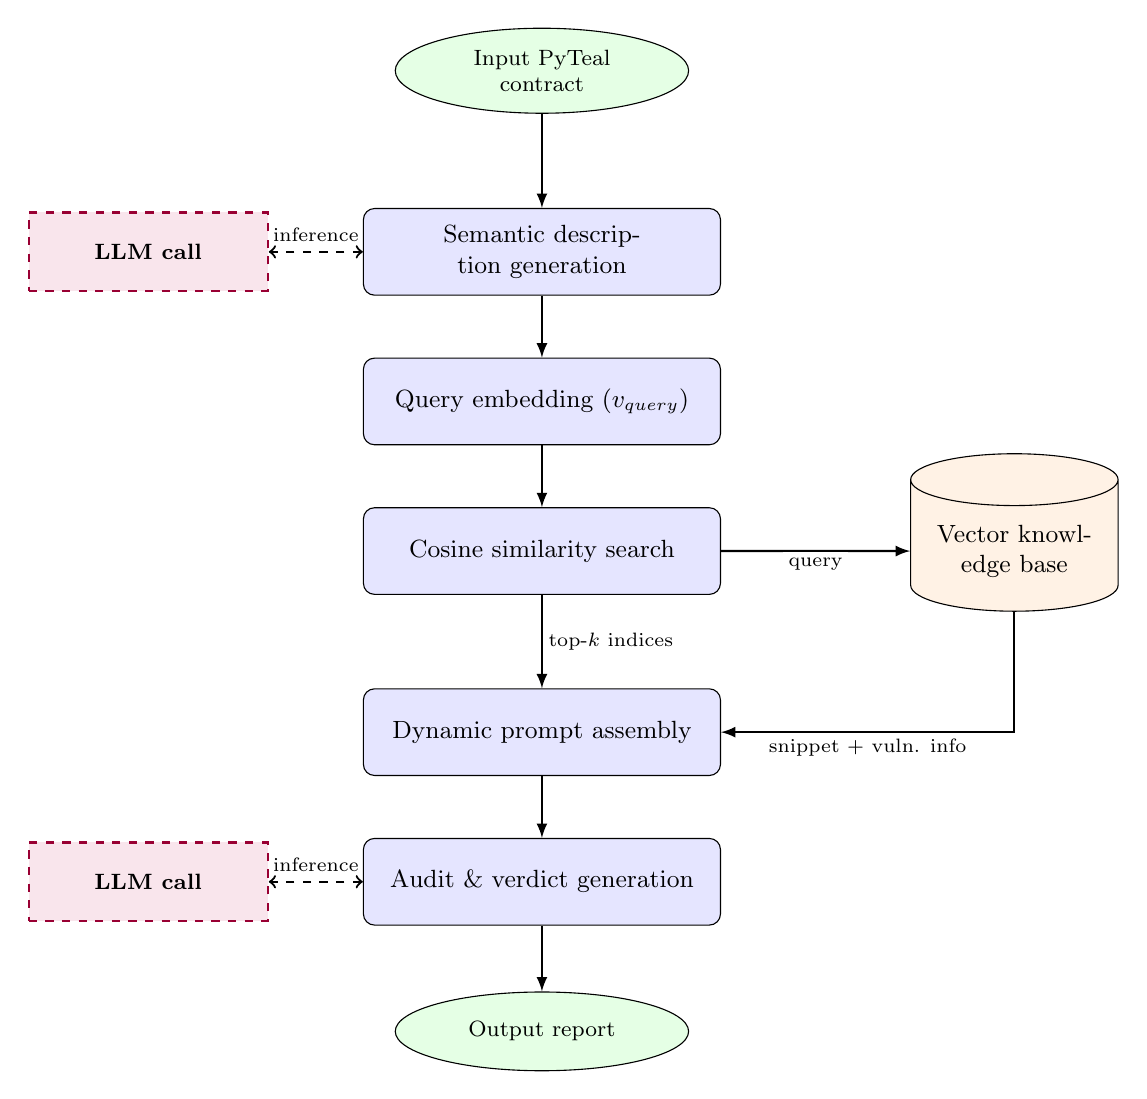
\begin{tikzpicture}[
        node distance=1.9cm,
        auto,
        block/.style={rectangle, draw, fill=blue!10, text width=4.3cm, text centered, rounded corners, minimum height=1.1cm, font=\small},
        cloud/.style={draw, ellipse, fill=green!10, minimum height=1cm, text width=2.4cm, text centered, font=\footnotesize},
        storage/.style={cylinder, draw, shape border rotate=90, aspect=0.25, fill=orange!10, text width=2.4cm, text centered, minimum height=2.0cm, font=\small},
        llm/.style={rectangle, draw=purple!80!black, fill=purple!10, thick, dashed, text width=2.8cm, text centered, minimum height=1cm, font=\footnotesize\bfseries},
        line/.style={draw, -latex, thick},
        description/.style={fill=white, inner sep=2pt, font=\scriptsize, align=center}
    ]
    \node [cloud] (input) {Input PyTeal contract};
    \node [block, below of=input, node distance=2.3cm] (desc_gen) {Semantic description generation};
    \node [block, below of=desc_gen, node distance=1.9cm] (embed) {Query embedding ($v_{query}$)};
    \node [block, below of=embed, node distance=1.9cm] (search) {Cosine similarity search};
    \node [block, below of=search, node distance=2.3cm] (prompt) {Dynamic prompt assembly};
    \node [block, below of=prompt, node distance=1.9cm] (audit_step) {Audit \& verdict generation};
    \node [cloud, below of=audit_step, node distance=1.9cm] (output) {Output report};
    \node [storage, right of=search, node distance=6cm] (vectorstore) {Vector knowledge base};
    \node [llm, left of=desc_gen, node distance=5cm] (llm_desc) {LLM call};
    \node [llm, left of=audit_step, node distance=5cm] (llm_audit) {LLM call};
    \path [line] (input) -- (desc_gen);
    \path [line] (desc_gen) -- (embed);
    \path [line] (embed) -- (search);
    \path [line] (search) -- node[description, pos=0.5] {top-$k$ indices} (prompt);
    \path [line] (prompt) -- (audit_step);
    \path [line] (audit_step) -- (output);
    \draw [line, dashed, <->] (desc_gen) -- node[above, font=\scriptsize] {inference} (llm_desc);
    \draw [line, dashed, <->] (audit_step) -- node[above, font=\scriptsize] {inference} (llm_audit);
    \draw [line] (search) -- node[description, below] {query} (vectorstore);
    \draw [line] (vectorstore) |- node[description, near end] {snippet + vuln. info} (prompt);
    \end{tikzpicture}
    \caption{Architecture of the proposed LLM-centric RAG pipeline. Dashed purple blocks denote LLM inference calls; the same underlying model is used for semantic-description generation and for the final audit step.}
    \label{fig:rag_architecture}
\end{figure}

Figure~\ref{fig:rag_architecture} shows the end-to-end pipeline. The model is invoked twice per contract: once to generate a syntax-agnostic semantic description used to query the vector store (Section~\ref{sec:sec_code_desc}), and once to produce the final audit, conditioned on a dynamically assembled prompt that combines the target code with retrieved context (Section~\ref{sec:retrieval_workflow}). Fine-tuning (Section~\ref{sec:finetuning_setup}) is designed so that the same model performs both roles well. The pipeline architecture, task schema, and training recipe below are language-agnostic; each is \emph{instantiated twice} -- once against the Algorand/PyTeal taxonomy of Table~\ref{tab:taxonomy}, once against a seven-class Solana/Rust taxonomy (Missing Key Check, Type Confusion, CPI Reentrancy, Unchecked External Calls, Integer Overflow, Bump Seed Canonicalization, and Denial of Service) -- with the concrete numbers for each instantiation given inline.

\subsection{Vulnerability Knowledge Base}
\label{sec:kb}

For each vulnerability class we curated a structured profile with four fields, populated identically for both languages: (i) a \emph{technical description} of the flaw in terms of the target virtual machine's execution semantics, (ii) the \emph{attack vector}, i.e., the concrete transaction or instruction pattern that triggers the exploit, (iii) the \emph{security check(s)} an auditor (or the model) must verify in the code, and (iv) a \emph{mitigation pattern} expressed as a canonical secure-coding idiom. For Algorand, these profiles were cross-validated against Trail of Bits' Algorand security documentation \citep{trailofbits_algorand} and the OWASP-mapped taxonomy of \citet{boi2025}; the Solana profiles were built analogously from the Sealevel attacks reference corpus and Anchor's documented account-constraint idioms. Table~\ref{tab:kb_examples} details four representative Algorand entries; the schema for Solana entries is identical, substituting AVM/transaction-field semantics with Sealevel account/instruction semantics (e.g., ``verify \texttt{signer} and \texttt{owner} constraints on every \texttt{AccountInfo}'' in place of ``verify \texttt{Txn.sender()}'').

\begin{table}[ht]
\centering
\small
\begin{tabular}{p{2.6cm}p{4.4cm}p{4.4cm}}
\toprule
\textbf{Class} & \textbf{Attack vector} & \textbf{Security check} \\
\midrule
Arbitrary Update / Delete & Attacker sends a transaction with \texttt{OnComplete} set to \texttt{UpdateApplication} or \texttt{DeleteApplication}; the contract exposes no sender check, so it replaces its own logic or destroys its state. & Presence of a branch handling \texttt{OnComplete.UpdateApplication}/\texttt{DeleteApplication} that asserts \texttt{Txn.sender()} == \texttt{Global.creator\_address()}. \\
\addlinespace
Unchecked (Asset) Receiver & Attacker injects, into a transaction group, a \texttt{Pay} or \texttt{Axfer} whose receiver field is their own address; the contract never validates it, so funds are diverted. & Every inner/group transaction's \texttt{Receiver}/\texttt{AssetReceiver} field is compared against an expected or whitelisted address. \\
\addlinespace
Unchecked RekeyTo & A LogicSig-approved transaction leaves \texttt{rekey\_to} unchecked; attacker sets it to their own address and takes over signing authority for the account. & Every non-\texttt{ApplCall} transaction asserts \texttt{Txn.rekey\_to() == Global.zero\_address()}. \\
\addlinespace
Unchecked Transaction Fee & Contract approves transactions without an upper bound on \texttt{fee}; attacker submits an excessive fee, draining the paying account via Algorand's fee-pooling mechanism. & An inequality check enforces \texttt{Txn.fee() <= Int(MAX\_FEE)}. \\
\bottomrule
\end{tabular}
\caption{Representative knowledge-base entries for the Algorand taxonomy (attack vector and required check fields only; the description and mitigation fields are omitted for space).}
\label{tab:kb_examples}
\end{table}

This knowledge base serves two purposes throughout the pipeline: it supplies the ground truth used to synthesize CoT training targets (Section~\ref{sec:cot_methodology}), and, independently, it populates the retrieval corpus consumed at inference time by the RAG module (Section~\ref{sec:rag_implementation}) -- the same four fields reappear verbatim inside the dynamic checklist injected into the audit prompt (Listing~\ref{lst:checklist_prompt}).

\subsection{Dataset Construction}
\label{sec:dataset_creation}

\subsubsection{Collection and vulnerability injection}
For Algorand, we collected 110 PyTeal smart contracts (100 for training, 10 held out for validation) from Algorand's official PyTeal repository \citep{algorand_pyteal_github}, covering DeFi/AMM protocols, escrow and atomic-swap services, recurring-payment logic signatures, and crowdfunding/governance contracts. To obtain matched vulnerable/safe pairs that isolate security-relevant differences from business-logic differences, we manually injected vulnerabilities into originally safe templates by removing or weakening the specific check listed in the corresponding knowledge-base profile (e.g., deleting the \texttt{Txn.sender()} assertion to produce an Arbitrary Delete instance), rather than sourcing unrelated vulnerable code. This produces contract pairs with near-identical business logic but opposite security profiles, forcing the model to attend to fine-grained security semantics rather than surface structure.

For Solana, we followed the same injection philosophy but sourced base instruction handlers from real, deployed Rust programs in the Solana Program Library and related open-source repositories (token-lending, \texttt{spl-governance}, stake-pool, escrow, and IDO-pool programs), rather than from templates written for this study, so that the resulting examples reflect production Anchor/native coding idioms rather than an artificial style. Vulnerable variants were produced by removing the specific account/signer/CPI check identified for each of the seven Solana classes; a small number of contrastive pairs (bump-seed canonicalization and type-cosplay) were additionally sourced from the \texttt{coral-xyz/sealevel-attacks} reference repository of known Solana exploit patterns.

\subsubsection{Composition}
The Algorand training corpus (100 contracts) is balanced as 80\% vulnerable samples (10\% per vulnerability class, eight classes) and 20\% safe samples; where authentic examples of a specific opcode combination were scarce, minimal synthetic snippets isolating the target pattern were added. An independent test set of 45 contracts (5 per vulnerability class, plus 5 safe contracts) was held out for final evaluation and is disjoint from the training and validation splits (Section~\ref{sec:test_set}).

The Solana corpus starts from 285 source contract pairs and, unlike the Algorand corpus, is constructed as \emph{per-vulnerability contrastive pairs} (a safe and a vulnerable variant of the same handler for each of the seven classes) rather than a single 80/20 vulnerable/safe split; targeted enrichment rounds -- driven by the failure analysis of Section~\ref{sec:results} -- added governance- and Anchor-framework-derived pairs plus additional Denial-of-Service and generically-safe examples, bringing the final training set to 267 instruction pairs (25 held out for validation). The held-out Solana test set was likewise grown, under continuous train/test leakage checks, from an initial 59 to 97 labeled contracts as failure modes were identified, to obtain a statistically sturdier and more class-balanced evaluation basis.

\subsubsection{Multi-task instruction schema}
\label{sec:training_tasks}
From the base contracts of each language we generated instruction-tuning instances spanning three tasks (approximately 500 for Algorand, from the 100 base contracts), so that the same underlying model can serve every stage of the pipeline in Figure~\ref{fig:rag_architecture}:
\begin{description}
\item[Task 1 -- Vulnerability detection.] Generic audit instruction (``perform a security audit of this contract''); the target response contains a \texttt{<think>} block with a step-by-step execution-flow analysis followed by a \texttt{<final>} verdict. This is the core CoT-reasoning task.
\item[Task 2 -- Targeted vulnerability verification.] The instruction names a specific hypothesis (e.g., ``check whether this contract is vulnerable to Unchecked RekeyTo''), and the target response verifies only that hypothesis, ignoring other potential defects. This trains the model to act as a \emph{hypothesis verifier}: at inference time, when the RAG checklist injects a ranked set of suspected vulnerabilities, the model activates this same focused-attention pattern to confirm or refute each suggestion in turn, rather than free-associating across the whole taxonomy.
\item[Task 3 -- Semantic code description.] The instruction requests a structured natural-language summary covering (a) architectural type (e.g., stateful application vs.\ stateless LogicSig for Algorand; on-chain program vs.\ CPI-invoked instruction handler for Solana), (b) functional intent (e.g., escrow, voting, marketplace, staking), and (c) validation logic -- which fields/accounts are checked and, critically, which are \emph{not}. Outputs from this task, generated with a fixed schema, are what gets indexed in the vector store, so consistency between indexing-time and query-time descriptions is critical (Section~\ref{sec:retrieval_workflow}).
\end{description}

\subsection{Chain-of-Thought Fine-Tuning}
\label{sec:cot_methodology}

Rather than framing training as binary code-to-label classification, target responses are engineered as a two-phase reasoning trace: a \texttt{<think>} phase, where the model scans the contract handler-by-handler (or instruction-by-instruction, for Solana), validating both insecure \emph{and} secure branches to build a complete audit context, and a \texttt{<final>} phase reporting the vulnerability name, a causal explanation, and a severity level (Critical/High/Medium/Low). This design follows the CoT literature showing that supervising intermediate reasoning steps improves performance on logic-heavy tasks \citep{wei2022chain}: rather than performing simple pattern matching against term frequencies seen in training, the model is forced to simulate a System-2-style reasoning process, decomposing the analysis into logical blocks (creation handler, administrative-operation handlers, per-instruction account checks) in a manner that emulates a human auditor. This is intended to reduce hallucination by forcing the model to state preconditions explicitly (e.g., ``is this a Smart Signature?'', ``does this instruction perform a CPI?'') before asserting a verdict, rather than jumping directly to a label. Listing~\ref{lst:cot_example} shows a representative Algorand training target for an Unchecked Asset Receiver instance.

\begin{lstlisting}[caption={Representative Chain-of-Thought training target (Unchecked Asset Receiver).}, label={lst:cot_example}]
<think>
Systematic analysis of the asset-transfer handler reached via the NoOp
branch.
1. Creation handler: correct, sender is stored as creator.
2. Update/Delete handlers: restricted to creator-only, no issue.
3. NoOp handler (critical path): validates argument presence and asset
   existence, but forwards `Txn.accounts[1]` directly as the transfer
   recipient without further checks.
4. Risk: `accounts` is attacker-supplied and unvalidated by the
   contract, so any caller can redirect the asset transfer to an
   arbitrary address.
</think>
<final>
The contract contains a critical vulnerability in the NoOp handler: the
asset receiver address is never validated, allowing an attacker to
drain the held assets.
### Vulnerability: Unchecked Asset Receiver
### Risk: Critical - total loss of assets held by the contract.
</final>
\end{lstlisting}

\subsubsection{Data efficiency}
\label{sec:dataset_limitations}
The resulting Algorand corpus ($\sim$500 instruction instances from 100 base contracts) is small relative to typical instruction-tuning corpora, and the Solana corpus (267 training pairs) is smaller still. We follow the ``quality-over-quantity'' alignment argument of LIMA \citep{zhou2023lima}: because each example encodes a dense, structured reasoning trace rather than a bare (input, label) pair, the model is not asked to learn the full distribution of PyTeal or Rust syntax from scratch (already present from pre-training) but to internalize a transferable \emph{auditing procedure} -- once the model has learned that ``the \texttt{rekey\_to} field must be checked,'' it tends to apply that rule to unseen contracts, which mitigates the effect of a small example count. RAG plays a complementary, compensatory role here: even where the model's parametric knowledge from a handful of fine-tuning examples is incomplete, retrieval supplies the missing contextual rule at inference time from the (larger, more easily extended) knowledge base rather than requiring it to be baked into model weights. We nonetheless treat corpus size, particularly on the Solana side, as a limitation requiring careful reporting, discussed in Section~\ref{sec:threats}.

\subsection{Model Selection}
\label{sec:model_selection}

We restrict model selection to the 32B parameter class, deliberately excluding smaller ($<$15B) and larger ($>$70B) open models. This choice is grounded in recent pretraining scaling-law analysis for reasoning \citep{wang2025larger}, which reports a non-monotonic (``U-shaped'') relationship between model size and the ability to infer multi-hop logical rules: the model size needed to avoid this failure mode grows linearly with the task's \emph{graph search entropy}. Both PyTeal auditing (multi-hop transaction-field and global-state dependencies) and Solana auditing (cross-instruction account flow and CPI-target validation) are high-entropy tasks in this sense -- undersized models lack the parametric density to map these latent rules and default to superficial syntactic pattern recognition. A preliminary qualitative pilot comparing 14B and 32B open models on the Algorand task corroborated this: 14B models showed adequate syntactic competence but repeatedly lost coherence mid-chain during CoT generation, while 32B models (Qwen3-32B, QwQ-32B) sustained a complete audit trace. Exploring the ascending branch of the curve (e.g., 70B+ models) is left to future work due to fine-tuning compute constraints (Section~\ref{sec:conclusion}).

Within the 32B class we fine-tuned Qwen3-32B for both languages, and additionally QwQ-32B for Algorand, on the basis of (i) native optimization, in the QwQ variant, for emitting intermediate reasoning before a final answer, which aligns with our \texttt{<think>}/\texttt{<final>} schema and reduces convergence time -- since the base model already segregates reasoning from answer, less capacity has to be spent learning that segregation from scratch -- and (ii) competitive code-intelligence benchmark performance within the 32B class for both models. The Solana instantiation of this study used Qwen3-32B only, to keep the cross-language comparison of Section~\ref{sec:results} centered on a single, shared base model.

\subsection{Fine-Tuning Configuration}
\label{sec:finetuning_setup}

Both Qwen3-32B and QwQ-32B were fine-tuned with QLoRA \citep{dettmers2023qlora,hu2021lora} using the Unsloth training framework. The base model was loaded in 4-bit NF4 quantization; LoRA adapters ($r=64$, $\alpha=128$) were attached to \emph{all} linear projections, including the MLP modules (\texttt{gate\_proj}, \texttt{up\_proj}, \texttt{down\_proj}) rather than only the attention projections, which we found necessary to meaningfully affect reasoning behavior rather than surface style. Full hyperparameters are listed in Table~\ref{tab:hyperparams}.

\begin{table}[!h]
\centering
\caption{Fine-tuning configuration.}
\label{tab:hyperparams}
\begin{tabular}{ll}
\toprule
\textbf{Parameter} & \textbf{Value} \\
\midrule
\multicolumn{2}{l}{\emph{Model and adaptation}} \\
\midrule
Base model & Qwen3-32B / QwQ-32B (Unsloth) \\
Quantization & 4-bit NF4 \\
PEFT method & QLoRA \\
LoRA rank ($r$) & 64 \\
LoRA alpha ($\alpha$) & 128 \\
Target modules & all linear layers (attention + MLP) \\
Dropout & 0.0 \\
\midrule
\multicolumn{2}{l}{\emph{Training dynamics}} \\
\midrule
Epochs & 3 \\
Effective batch size & 8 (1 per device $\times$ 8 grad. accum.) \\
Learning rate & $5\times 10^{-5}$ \\
Scheduler & cosine, 5\% warmup \\
Optimizer & paged AdamW (8-bit) \\
Max sequence length & 2048 tokens \\
Weight decay & 0.02 \\
Gradient checkpointing & enabled \\
Seed & 3407 \\
\bottomrule
\end{tabular}
\end{table}

\subsubsection{Chat template and loss masking}
A custom Jinja2 chat template was injected into the tokenizer to (i) enforce ChatML-style role boundaries between \texttt{system}, \texttt{user}, and \texttt{assistant} turns via the \texttt{<|im\_start|>}/\texttt{<|im\_end|>} special tokens, (ii) introduce the \texttt{<think>}/\texttt{<final>} segregation as first-class template constructs, ensuring the model always emits the reasoning block before the verdict rather than answering impulsively, and (iii) branch conditionally between the CoT schema (Tasks 1--2, which populate a \texttt{thinking} field) and the direct-answer schema (Task 3, which populates only a \texttt{description} field). Loss was computed only over response tokens (\texttt{train\_on\_responses\_only}, splitting instruction from response at the \texttt{<|im\_start|>user}/\texttt{<|im\_end|>} boundary), masking the fixed instruction/code portion of each example. This has two effects: it focuses gradient updates exclusively on the tokens the model must learn to produce (the reasoning trace and the verdict), accelerating convergence toward the target behavior, and it prevents the model from memorizing incidental phrasing in the fixed instruction/code portion of the prompt, reducing the risk of format-specific overfitting.

\subsubsection{Early stopping}
\label{sec:loss_analysis}
Training and validation loss were logged every 10 steps over 3 epochs (180 steps) for the Algorand models. Table~\ref{tab:loss_curve} reports loss at selected checkpoints. Both models show rapid joint convergence over the first 100 steps (train loss $\sim1.4\rightarrow\sim0.6$), indicating the models are learning the CoT syntax and PyTeal-specific structure effectively, with validation loss following the same trend (confirming the learning generalizes rather than merely memorizing). Beyond step 120--130 a generalization gap opens: training loss for QwQ-32B continues to fall monotonically (to 0.51 at step 150), consistent with the model beginning to memorize training-set-specific details, while validation loss plateaus for Qwen3-32B ($\sim0.555$) and mildly \emph{increases} for QwQ-32B ($0.562\rightarrow0.582$ between steps 90 and 180) -- the onset of overfitting. QwQ-32B's greater sensitivity to this effect is consistent with its specialization for reasoning, which appears to make it more prone to fitting spurious reasoning-trace idiosyncrasies of the (comparatively small) training set. We therefore fixed training at 3 epochs for both models, stopping at the empirical validation-loss optimum -- the ``Goldilocks zone'' where reasoning capability has been acquired but predictive degradation on unseen contracts has not yet begun -- rather than continuing to minimize training loss.

\begin{table}[!h]
\centering
\small
\caption{Training/validation loss at selected checkpoints (Algorand fine-tuning).}
\label{tab:loss_curve}
\begin{tabular}{lcccccc}
\toprule
& \multicolumn{6}{c}{Step} \\
\cmidrule(lr){2-7}
& 10 & 50 & 90 & 130 & 150 & 180 \\
\midrule
Qwen3-32B (train) & 1.323 & 0.761 & 0.592 & 0.577 & 0.496 & 0.514 \\
Qwen3-32B (val)   & 0.803 & 0.598 & 0.566 & 0.554 & 0.568 & 0.565 \\
QwQ-32B (train)   & 1.426 & 0.790 & 0.606 & 0.587 & 0.503 & 0.518 \\
QwQ-32B (val)     & 0.821 & 0.611 & 0.583 & 0.565 & 0.583 & 0.579 \\
\bottomrule
\end{tabular}
\end{table}

\subsection{Retrieval-Augmented Generation Pipeline}
\label{sec:rag_implementation}

\subsubsection{Knowledge base construction}
The Algorand RAG corpus indexes 40 vulnerable contracts (5 per class), distinct from the training and test splits; the Solana RAG corpus indexes 38 entries across the seven classes, including a dedicated re-initialization-guard entry for Denial of Service added during the failure-driven diagnosis of Section~\ref{sec:results} to close a coverage gap in that category. Each entry stores three fields: a \emph{vulnerability label} (metadata, linking to the profile in Section~\ref{sec:kb}), a \emph{semantic description} (the field actually embedded and searched, produced with the Task-3 schema of Section~\ref{sec:training_tasks}), and a \emph{vulnerable snippet} (payload, not embedded, injected verbatim as a few-shot example once retrieved). Descriptions were embedded with \texttt{hkunlp/instructor-xl} into dense vectors used purely for the cosine-similarity search of Section~\ref{sec:retrieval_workflow}; the snippet payload itself never enters the embedding space.

\subsubsection{Semantic-abstraction retrieval}
\label{sec:sec_code_desc}
Indexing raw code risks clustering contracts by \emph{application domain} (all auctions near each other, all voting contracts near each other, all staking programs near each other) rather than by \emph{security profile}, since two functionally identical contracts can differ entirely in which checks they omit -- the same raw-code retrieval bias documented for Vul-RAG \citep{vulrag2024}. We instead index an LLM-generated description constrained by two directives: (i) \emph{syntactic abstraction} -- omit variable names, literals, and comments, which are retrieval noise that separates contracts implementing the same security logic in different coding styles; and (ii) \emph{security-check mapping} -- explicitly enumerate which fields/accounts are validated and, critically, which are \emph{not} (e.g., ``no explicit check on the \texttt{RekeyTo} field of the payment transaction'' for Algorand, or ``the CPI target program ID is never validated before invocation'' for Solana). This shifts the embedding space toward a representation of the \emph{vulnerability structure} rather than the \emph{contract function}: the retrieval question being answered is not ``what does this contract do?'' but ``does this contract exhibit patterns overlapping a known vulnerability?'', increasing the likelihood that retrieval surfaces an example sharing the same underlying flaw rather than merely the same application domain.

\subsubsection{Retrieval and diversification workflow}
\label{sec:retrieval_workflow}
Rather than a simple keyword search, querying the knowledge base follows a four-phase pipeline, illustrated end to end in Figure~\ref{fig:rag_architecture}:
\begin{description}
\item[Phase 1 -- Description generation.] The model under test is prompted to produce a Task-3 description of the target contract, using the identical schema and instructions used at indexing time. This consistency requirement is not incidental: any drift between the indexing-time and query-time description style shifts the query vector out of the region of embedding space the knowledge base was populated in, degrading retrieval quality regardless of how good the underlying embedding model is.
\item[Phase 2 -- Embedding and similarity ranking.] The generated description is embedded with the same model used for indexing, producing a query vector $v_{query}$; the pipeline computes cosine similarity $\mathrm{Sim}(v_{query}, v_{doc})$ against every knowledge-base entry and produces a ranked candidate list.
\item[Phase 3 -- Selection and diversification.] Rather than taking the top-$N$ candidates by raw score -- which risks returning $N$ near-duplicate examples of the same vulnerability -- the pipeline greedily selects the single best match, then walks down the ranked list discarding any candidate whose vulnerability label duplicates one already selected, until $N$ \emph{distinct} vulnerability classes are represented. This guarantees the final context spans a variety of plausible threats rather than over-covering one.
\item[Phase 4 -- Context injection.] The vulnerable-snippet payload and technical description of each of the $N$ selected candidates are injected into the system prompt as few-shot context, following the few-shot in-context-learning paradigm: the model is shown concrete examples of ``what a similar flaw looks like'' in the code it is about to analyze, anchoring its attention on specific patterns instead of relying solely on parametric memory.
\end{description}

\subsubsection{Dynamic checklist prompting}
\label{sec:prompt_engineering}
Rather than asking the model to ``find any bug,'' the prompt enumerates every vulnerability class in the taxonomy as an ordered checklist, re-ranked per contract by the retrieval step above: the top-$N$ retrieved classes are placed first, annotated with their similarity score and full technical detail (description, precondition, check, vulnerable-pattern example), signaling to the model that these are the most probable issues and should be verified first, while the remaining classes are appended in abbreviated (name-only) form so that low-similarity categories are never silently dropped from consideration -- even a weak retrieval signal still triggers a baseline check for every class in the taxonomy. Listing~\ref{lst:checklist_prompt} shows a representative excerpt. Showing full detail only for the top-$N$ matches, rather than for the entire taxonomy, is a deliberate context-budget tradeoff: including every class's full description and vulnerable-pattern example risks diluting the model's attention across too many code snippets, making it harder to distinguish the target contract from the retrieved examples, whereas concentrating detail on the few most relevant matches keeps the prompt focused. $N$ was set to 3 for Algorand, matching the 32B context-window budget used in that instantiation; for Solana, $N$ was determined empirically via a checklist-size ablation sweeping $N \in \{0, \ldots, 7\}$ against held-out accuracy (Section~\ref{sec:results}), which identified $N=2$ as optimal for that language's taxonomy and test distribution -- underscoring that this hyperparameter is language- and corpus-dependent rather than a fixed architectural constant. The design is intended to scale to larger $N$ with longer-context models.

\begin{lstlisting}[caption={Excerpt of a dynamically re-ranked checklist injected into the audit prompt.}, label={lst:checklist_prompt}]
-------------------------------- Checklist ---------------------------------
1. Arbitrary delete (score: 0.9255)
   Description: unrestricted DeleteApplication allows contract destruction.
   Precondition: stateful application handling DeleteApplication.
   Security check: restrict DeleteApplication to creator/admin.

2. Arbitrary update (score: 0.9101)
   Description: unrestricted UpdateApplication allows logic replacement.
   Precondition: handling of OnComplete.UpdateApplication.
   Security check: verify Txn.sender() == Global.creator_address().

3. Unchecked Asset Receiver (score: 0.9079)
   [... full detail for top-N matches ...]

4-8. [remaining classes, condensed]
------------------------------------------------------------------------
Audit instructions: use the list above as a priority guide. Analyze the
code step by step inside <think>, checking each precondition in order.
\end{lstlisting}

\subsection{Fine-Tuning versus SOTA Generalist Models: Rationale}
\label{sec:finetuning_rationale}

Before presenting results, it is worth stating explicitly the question this design is meant to answer, since it motivates the benchmark of Section~\ref{sec:experiments}. In the current landscape, dominated by massive-scale generalist LLMs (GPT-5, Claude, DeepSeek), the prevailing trend is to rely on these models' broad generalization ability through prompt engineering alone, avoiding the cost and complexity of fine-tuning. This raises a legitimate question: \emph{is it still worth fine-tuning a ``small'' (32B) model on a specific domain, or do massive generalist models render the practice obsolete?}

The two approaches offer opposite competitive advantages. The \emph{generalist} approach benefits from immense parametric knowledge and superior raw reasoning ability, adaptable to a new task purely through prompt instructions with no weight updates -- but it operates without any domain-specific practical experience: a generalist model may know PyTeal or Anchor syntax without having internalized the specific security nuances that come from focused exposure to that ecosystem's exploit patterns. The \emph{specialist} approach starts from weaker raw reasoning capacity at 32B parameters, but is intensively exposed, through the CoT corpus of Section~\ref{sec:dataset_creation}, to exactly the audit procedure and vulnerability patterns relevant to the task; the hypothesis is that this specialization can compensate for the smaller scale, letting the small model recognize patterns a generalist misses, or recognize them more reliably.

Independently of which approach wins on raw performance, fine-tuning a locally deployable model retains value along two non-functional dimensions relevant to real-world adoption. First, \textbf{data sovereignty}: using a massive generalist model in practice almost always means routing proprietary contract code through a third-party cloud API; for financial smart contracts still under trade-secret protection prior to deployment, this is frequently an unacceptable exposure, whereas a fine-tuned 32B model can be run entirely on-premise on commodity enterprise hardware. Second, \textbf{structural determinism}: generalist models, however capable, are more prone to verbosity or occasional drift from a requested output format, whereas a fine-tuned model has internalized the required structure (the \texttt{<think>}/\texttt{<final>} schema) in its weights, which matters for integration into an automated pipeline that parses the model's verdict downstream. The benchmark against DeepSeek-V3.2 in Section~\ref{sec:results} is designed to make this comparison concrete for the Algorand instantiation of the pipeline.

\section{Experimental Setup}
\label{sec:experiments}

\subsection{Models and Configurations}
\label{sec:exp_setup}
For \textbf{Algorand}, we evaluate five configurations spanning three model categories: (i) \emph{non-fine-tuned baselines}, Qwen3-32B and QwQ-32B as released; (ii) \emph{fine-tuned specialists}, Qwen3-32B-FT and QwQ-32B-FT, obtained via the procedure in Section~\ref{sec:finetuning_setup}; and (iii) a \emph{SOTA generalist}, DeepSeek-V3.2 (accessed via API), a $>$600B-parameter mixture-of-experts model representative of the current open-weights frontier, used purely through in-context learning (no fine-tuning). Each of the five configurations is tested both \emph{without} RAG (direct prompting; measures parametric knowledge alone) and \emph{with} RAG (Section~\ref{sec:rag_implementation}; measures the ability to exploit non-parametric context), for ten model$\times$retrieval combinations in total.

For \textbf{Solana}, we evaluate the narrower two-by-two design of base vs.\ fine-tuned Qwen3-32B, each without and with RAG, for four combinations; no SOTA-generalist benchmark was run for this language, and the RAG configuration was additionally swept over the checklist size $k$ (Section~\ref{sec:solana_results}) rather than fixed a priori, since no equivalent sweep had previously been run for this instantiation of the pipeline.

\subsection{Test Set}
\label{sec:test_set}
Algorand evaluation uses a held-out set of 45 contracts never seen during training or RAG-corpus construction: 40 vulnerable contracts (5 per class, each with a single verified ground-truth vulnerability) and 5 safe contracts, used to measure the false-positive/hallucination rate on code that contains no injected flaw.

The Solana test set began this study at 59 contracts and was expanded to 97 over the course of the experiments reported in Section~\ref{sec:solana_results}: an early bootstrap 95\% confidence interval on F1, computed on the smaller set, spanned approximately $[0.32, 0.65]$ -- wider than most of the point differences under investigation, since several vulnerability categories had only 4--7 labeled examples. Every added contract is real, previously unused code, individually read and hand-labeled, and verified by exact-string search to be absent from both the training set and the pre-existing test set before inclusion (a candidate public dataset, \texttt{ArmurAI/Solana\_vulnerability\_audit\_dataset\_V2}, was evaluated and rejected for this purpose, as its labels reflect generic Solidity/DeFi categories that do not correspond to Solana's threat model). Even at 97 contracts, per-category counts (6--9 examples) remain small enough that individual misclassifications materially affect reported per-category recall.

\subsection{Evaluation Metrics}
\label{sec:metrics}
Each model output is classified against ground truth as a True Positive (correct vulnerability identified), False Negative (contract declared safe, or the wrong vulnerability reported, when a flaw is present), False Positive (a vulnerability reported on a safe contract, or an additional, non-existent vulnerability reported alongside/instead of the correct one), or True Negative (a safe contract correctly declared safe). From these we compute standard detection metrics:
\begin{align}
\text{Accuracy} &= \frac{TP+TN}{TP+TN+FP+FN}, &
\text{Precision} &= \frac{TP}{TP+FP}, \\
\text{Recall} &= \frac{TP}{TP+FN}, &
F_1 &= 2\cdot\frac{\text{Precision}\cdot\text{Recall}}{\text{Precision}+\text{Recall}}.
\end{align}
In a security-audit context, recall is arguably the more critical metric, since a false negative corresponds to a missed exploitable bug, whereas low precision mainly costs auditor time ("alert fatigue").

\subsection{Automated Evaluation Pipeline}
\label{sec:eval_pipeline}
Given the combinatorial size of the benchmark (45 contracts $\times$ 10 configurations), we built an automated Python evaluation harness. Model output is parsed via a regular expression targeting the \texttt{<final>} block; if the tag is missing or malformed, the prompt is resubmitted up to three times before the response is discarded, so that reported metrics reflect reasoning ability rather than incidental formatting failures. The extracted verdict is then automatically compared against the ground-truth label to populate the TP/FP/FN/TN registry from which all metrics are derived (Figure~\ref{fig:eval_pipeline}). The same harness, with a language-appropriate parser, is used for the Solana instantiation of the pipeline. Section~\ref{sec:manual_verification} reports an independent, hand-scored audit of raw model outputs for both languages, run specifically to check whether this automated parsing step itself biases the reported metrics.

\begin{figure}[!h]
    \centering
    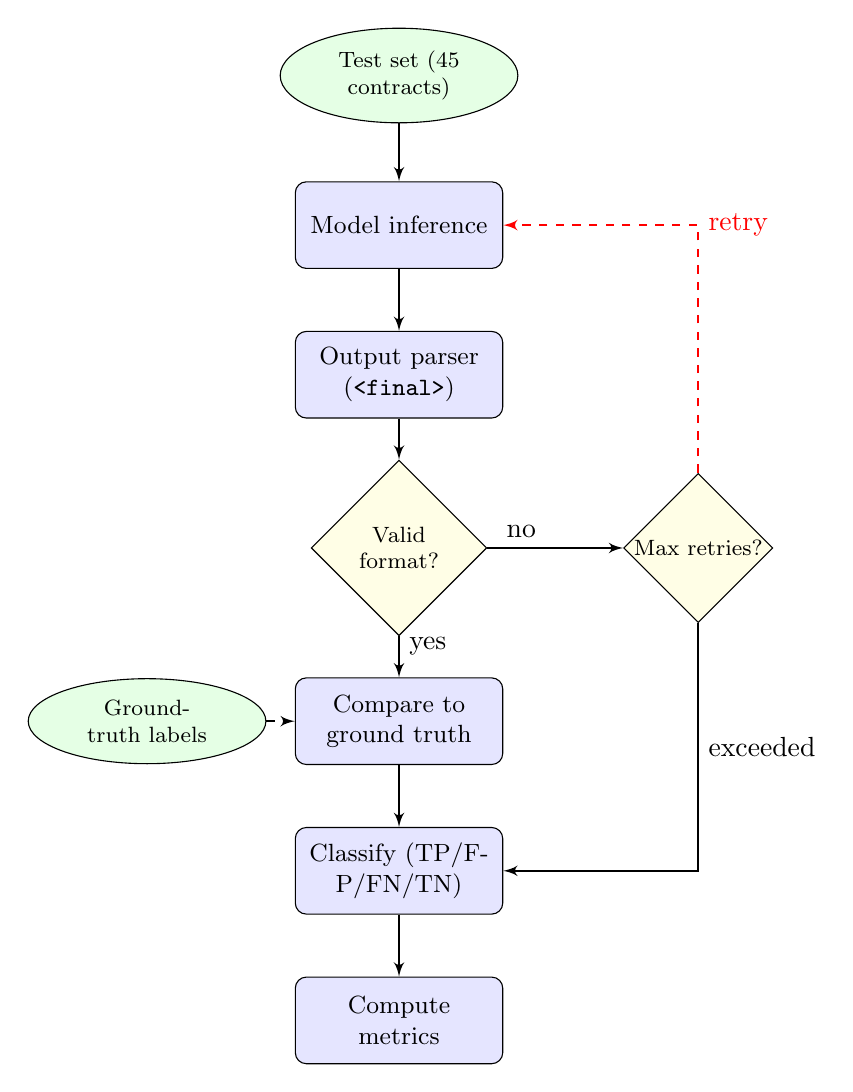
\begin{tikzpicture}[
        node distance=1.9cm, auto,
        block/.style={rectangle, draw, fill=blue!10, text width=2.4cm, text centered, rounded corners, minimum height=1.1cm, font=\small},
        decision/.style={diamond, draw, fill=yellow!10, text width=1.7cm, text centered, inner sep=0pt, font=\footnotesize},
        cloud/.style={draw, ellipse, fill=green!10, minimum height=0.8cm, text width=1.9cm, text centered, font=\footnotesize},
        line/.style={draw, -latex', thick},
        retry/.style={draw, -latex', thick, red, dashed}
    ]
    \node [cloud] (dataset) {Test set (45 contracts)};
    \node [block, below of=dataset] (inference) {Model inference};
    \node [block, below of=inference] (parser) {Output parser (\texttt{<final>})};
    \node [decision, below of=parser, node distance=2.2cm] (check) {Valid format?};
    \node [block, below of=check, node distance=2.2cm] (comparator) {Compare to ground truth};
    \node [decision, right of=check, node distance=3.8cm] (limit) {Max retries?};
    \node [block, below of=comparator] (classify) {Classify (TP/FP/FN/TN)};
    \node [block, below of=classify] (metrics) {Compute metrics};
    \path [line] (dataset) -- (inference);
    \path [line] (inference) -- (parser);
    \path [line] (parser) -- (check);
    \path [line] (check) -- node [near start, right] {yes} (comparator);
    \path [line] (check) -- node [near start, above] {no} (limit);
    \path [retry] (limit) |- node [right] {retry} (inference);
    \path [line] (limit) |- node [near start, right] {exceeded} (classify);
    \node [cloud, left of=comparator, node distance=3.2cm] (truth) {Ground-truth labels};
    \path [line, dashed] (truth) -- (comparator);
    \path [line] (comparator) -- (classify);
    \path [line] (classify) -- (metrics);
    \end{tikzpicture}
    \caption{Automated evaluation pipeline.}
    \label{fig:eval_pipeline}
\end{figure}

\section{Results}
\label{sec:results}

All results below are obtained under the stochastic decoding settings actually used at inference time (temperature 0.6, top-$p$ 0.95, sampling enabled) rather than the greedy decoding that an earlier, uncorrected version of the evaluation harness silently fell back to (Section~\ref{sec:rq5_stability} documents this correction and its effect). Every reported score is therefore a mean over $N=5$ independently seeded samples per configuration, with the sample-to-sample standard deviation reported alongside it; DeepSeek-V3.2, evaluated only through a metered third-party API, is the sole exception and is reported as a single run. The following subsections build up the evidence needed to answer RQ1 and RQ2 (Section~\ref{sec:intro}), with the two questions answered explicitly in Section~\ref{sec:results_summary}.

\subsection{Impact of Chain-of-Thought Fine-Tuning}
\label{sec:impact_finetuning}

Table~\ref{tab:confusion_matrix_raw} reports mean confusion-matrix counts (averaged over 5 seeded samples) for base and fine-tuned models under direct (no-RAG) prompting. Figure~\ref{fig:ft_impact_metrics} shows the derived metrics with their sample-to-sample standard deviation as error bars.

\begin{table}[!h]
\centering
\caption{Mean confusion-matrix counts over 5 seeded samples, base vs.\ fine-tuned models, no RAG (test set: 45 contracts).}
\label{tab:confusion_matrix_raw}
\resizebox{\textwidth}{!}{%
\begin{tabular}{l|cccc|c}
\toprule
\textbf{Model} & \textbf{TP} & \textbf{TN} & \textbf{FP} & \textbf{FN} & \textbf{Total} \\
\midrule
Qwen3-32B (base) & 17.0 & 1.6 & 18.2 & 23.0 & 59.8$^{*}$ \\
\textbf{Qwen3-32B (FT)} & \textbf{24.4} & \textbf{0.8} & \textbf{15.4} & \textbf{15.6} & 56.2$^{*}$ \\
\midrule
QwQ-32B (base) & 11.6 & 4.4 & 2.8 & 28.4 & 47.2$^{*}$ \\
\textbf{QwQ-32B (FT)} & \textbf{21.4} & \textbf{3.4} & \textbf{6.2} & \textbf{18.6} & 49.6$^{*}$ \\
\bottomrule
\end{tabular}%
}
\vspace{0.15cm}
\begin{minipage}{\textwidth}
\small $^{*}$Totals exceed 45 when a model reports multiple (or spurious) vulnerabilities on the same contract, each counted as a separate FP.
\end{minipage}
\end{table}

\begin{figure}[h]
    \centering
    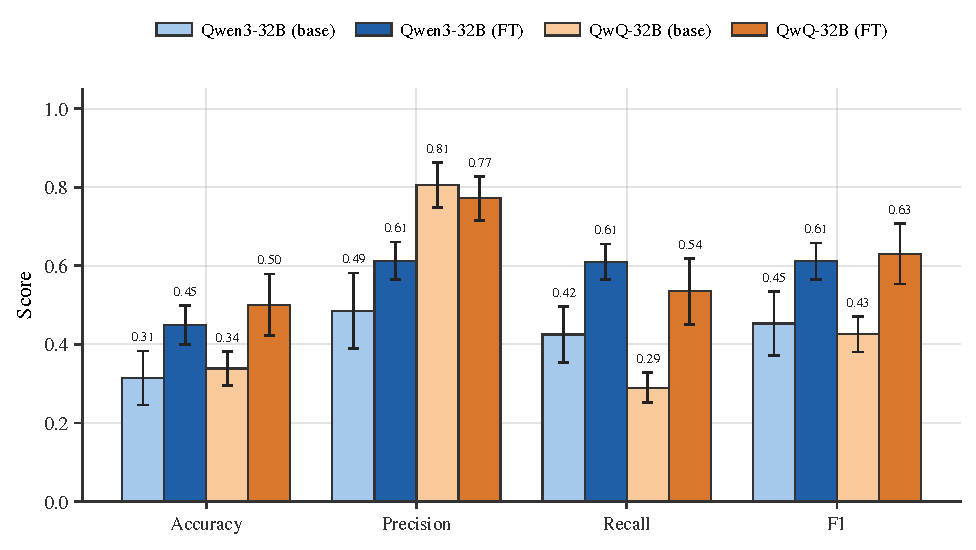
\includegraphics[width=0.85\textwidth]{../images/ft_impact_algorand.pdf}
    \caption{Effect of fine-tuning on Accuracy, Precision, Recall, and F1-score, no RAG (Algorand, 45-contract test set), mean $\pm$ std over 5 seeded samples. Fine-tuning improves every metric for both models on average; QwQ-32B shows the larger, but noisier, recall gain.}
    \label{fig:ft_impact_metrics}
\end{figure}

Fine-tuning affects precision and recall through distinct mechanisms, though both are noisier under proper sampling than a single greedy run would suggest. On the \emph{precision} axis, base Qwen3-32B suffers from a high false-positive rate (mean 18.2 FP over 45 contracts, precision 0.486$\pm$0.096); fine-tuning reduces this to a mean 15.4 FP, lifting precision to 0.613$\pm$0.047 -- a real but noisier gain than a single-run comparison would show, and evidence against the hypothesis that CoT fine-tuning on $\sim$500 examples would simply overfit and increase spurious detections. On the \emph{recall} axis, the reasoning-oriented QwQ-32B benefits most: the base model misses AVM-specific patterns at a high rate (mean 28.4 FN, recall 0.290$\pm$0.038), while fine-tuning raises recall to 0.535$\pm$0.084 by teaching the model to search for the \emph{absence} of specific checks rather than pattern-match superficial cues -- the largest relative gain observed, but also the noisiest (std 0.084), so individual anecdotal comparisons between the two models should be read with caution. Jointly, F1-score for Qwen3-32B improves from 0.453$\pm$0.082 (base) to 0.612$\pm$0.046 (fine-tuned), and for QwQ-32B from 0.426$\pm$0.045 to 0.631$\pm$0.077.

\subsubsection{Qualitative case study}
\label{sec:case_study_rekey}
To illustrate the mechanism behind this gain, consider a stateless (LogicSig) contract authorizing a two-transaction group: \texttt{Gtxn[0]} (payment) and \texttt{Gtxn[1]} (asset transfer). The contract is vulnerable because \texttt{Gtxn[1]} checks \texttt{rekey\_to}, but \texttt{Gtxn[0]} does not. The base Qwen3-32B model observes, correctly, that \texttt{rekey\_to} is checked in \texttt{Gtxn[1]}, but then over-generalizes this local observation to the whole contract, concluding "\emph{all relevant security checks are explicitly implemented for ... rekey\_to}" -- a textbook generalization hallucination that conflates a locally present check with global safety. The fine-tuned model instead maintains a per-transaction ledger of checks (\emph{"Payment Transaction (Gtxn[0]): ... Missing check: no validation of rekey\_to() field"}), correctly isolating the omission and reporting \emph{Unchecked RekeyTo} as the verdict. This indicates that fine-tuning does not merely add syntactic vocabulary but shifts the model's attention pattern from a "summarizing" read of the contract to a per-transaction "verifying" read.

\subsection{Benchmark Against a SOTA Generalist Model}
\label{sec:benchmark_deepseek}

Table~\ref{tab:sota_comparison} compares the best fine-tuned specialist (Qwen3-32B-FT, mean over 5 seeded samples) against DeepSeek-V3.2 (single run, API-metered) under direct prompting (no RAG for either model).

\begin{table}[!h]
\centering
\caption{Fine-tuned specialist (mean $\pm$ std, $N=5$) vs.\ SOTA generalist (single run), no RAG (test set: 45 contracts).}
\label{tab:sota_comparison}
\resizebox{\textwidth}{!}{%
\begin{tabular}{l|cccc}
\toprule
\textbf{Model} & \textbf{Precision} & \textbf{Recall} & \textbf{F1} & \textbf{Accuracy} \\
\midrule
Qwen3-32B (FT) & 0.613$\pm$0.047 & 0.610$\pm$0.045 & 0.612$\pm$0.046 & 0.450$\pm$0.049 \\
\textbf{DeepSeek-V3.2 (API)} & \textbf{0.717} & \textbf{0.825} & \textbf{0.767} & \textbf{0.649} \\
\bottomrule
\end{tabular}%
}
\end{table}

Under proper stochastic sampling and the corrected evaluation pipeline (Section~\ref{sec:rq5_stability}), a $>$600B-parameter generalist accessed purely through in-context learning outperforms the fine-tuned 32B specialist on every metric \emph{without} retrieval augmentation -- the reverse of what a single, uncorrected greedy run had suggested. This revises our earlier conclusion \citep{boi2025} that fine-tuning alone closes the gap to a generalist twenty times larger: at this stage of the pipeline (no RAG), it does not. Section~\ref{sec:rag_impact_analysis} shows that the picture changes substantially once retrieval is added to both models.

\subsection{Impact of Retrieval-Augmented Generation}
\label{sec:rag_impact_analysis}

Table~\ref{tab:rag_comparison_full} reports mean precision, recall, and F1 (with std over 5 seeded samples) with and without RAG for all five configurations; DeepSeek-V3.2 rows remain single-run.

\begin{table}[!h]
\centering
\caption{Impact of RAG on Precision, Recall, and F1-score, mean $\pm$ std over 5 seeded samples ($N=5$; DeepSeek-V3.2 is a single run). Values in parentheses are the net gain ($\Delta$) over the no-RAG condition.}
\label{tab:rag_comparison_full}
\resizebox{\textwidth}{!}{%
\begin{tabular}{l|cc|cc|cc}
\toprule
\textbf{Model} & \multicolumn{2}{c|}{\textbf{Precision}} & \multicolumn{2}{c|}{\textbf{Recall}} & \multicolumn{2}{c}{\textbf{F1}} \\
 & No-RAG & With RAG & No-RAG & With RAG & No-RAG & With RAG \\
\midrule
\multicolumn{7}{l}{\emph{Base models}} \\
QwQ-32B & 0.805$\pm$0.058 & \textbf{0.878$\pm$0.023 (+0.073)} & 0.290$\pm$0.038 & \textbf{0.710$\pm$0.042 (+0.420)} & 0.426$\pm$0.045 & \textbf{0.784$\pm$0.021 (+0.358)} \\
Qwen3-32B & 0.486$\pm$0.096 & \textbf{0.742$\pm$0.039 (+0.256)} & 0.425$\pm$0.071 & \textbf{0.730$\pm$0.048 (+0.305)} & 0.453$\pm$0.082 & \textbf{0.735$\pm$0.038 (+0.282)} \\
\midrule
\multicolumn{7}{l}{\emph{Fine-tuned models}} \\
QwQ-32B (FT) & 0.772$\pm$0.056 & \textbf{0.819$\pm$0.024 (+0.047)} & 0.535$\pm$0.084 & \textbf{0.810$\pm$0.029 (+0.275)} & 0.631$\pm$0.077 & \textbf{0.814$\pm$0.014 (+0.183)} \\
\textbf{Qwen3-32B (FT)} & 0.613$\pm$0.047 & \textbf{0.792$\pm$0.059 (+0.179)} & 0.610$\pm$0.045 & \textbf{0.805$\pm$0.021 (+0.195)} & 0.612$\pm$0.046 & \textbf{0.798$\pm$0.036 (+0.186)} \\
\midrule
\multicolumn{7}{l}{\emph{SOTA generalist (single run)}} \\
DeepSeek-V3.2 & 0.717 & \textbf{0.91 (+0.19)} & 0.825 & \textbf{0.97 (+0.15)} & 0.767 & \textbf{0.94 (+0.17)} \\
\bottomrule
\end{tabular}%
}
\end{table}

\begin{figure}[h!]
    \centering
    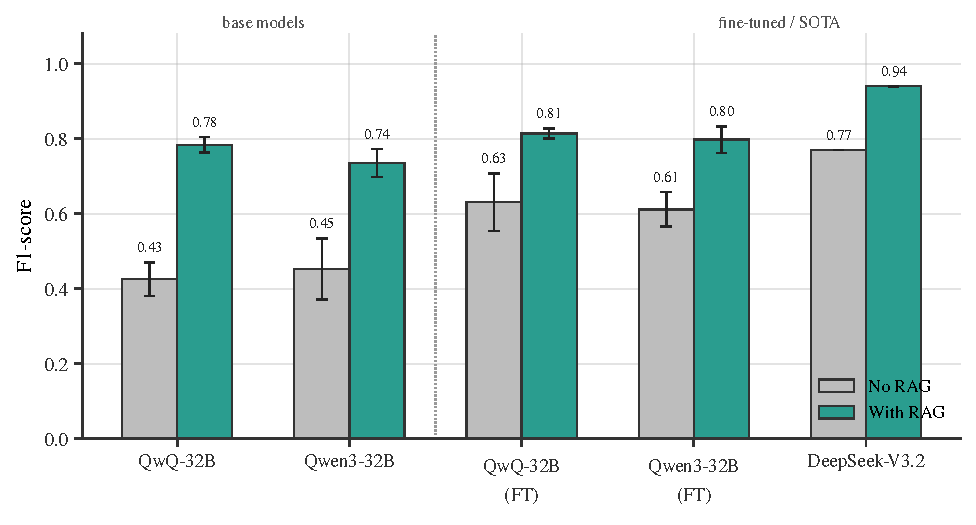
\includegraphics[width=0.85\textwidth]{../images/rag_impact_algorand.pdf}
    \caption{F1-score without vs.\ with RAG, all five Algorand configurations, mean $\pm$ std over 5 seeded samples (DeepSeek-V3.2 single run). RAG is additive for every configuration, base models included; the gap to the SOTA generalist (DeepSeek-V3.2) shrinks from 0.13--0.34 F1 (no RAG) to 0.13--0.16 F1 (with RAG) once fine-tuning is applied to the 32B models.}
    \label{fig:rag_impact_all}
\end{figure}

RAG improves mean F1-score in every configuration tested, but through different mechanisms depending on model maturity. For \emph{base} models, retrieval acts primarily as a \emph{noise filter}: grounding the model in real retrieved examples sharply curbs hallucinated findings, raising Qwen3-32B precision from 0.486$\pm$0.096 to 0.742$\pm$0.039, and raises recall as well (0.425$\pm$0.071 to 0.730$\pm$0.048), unlike the earlier uncorrected run, which had shown a spurious small recall drop. For \emph{fine-tuned} models, we observe the most favorable synergy: prior training supplies syntactic and procedural competence, while RAG extends effective "memory" with concrete, on-demand examples, jointly raising QwQ-32B-FT to a mean F1 of 0.814$\pm$0.014 -- our most stable configuration (lowest std of any Algorand result) and a strong, on-premise-deployable result. For the \emph{SOTA generalist} DeepSeek-V3.2, RAG still closes a residual domain gap, pushing recall to 0.97 (39/40, a single missed vulnerability) and F1 to 0.94, indicating that even massive parametric knowledge does not saturate performance on a low-resource language like PyTeal without external grounding; because this figure is a single run, it cannot itself be checked for sampling stability the way the other rows can.

Three patterns are consistent across the full table. First, \textbf{RAG is uniformly additive on average}: no configuration's mean F1-score degrades when retrieval is added, and every gain is comfortably larger than the corresponding standard deviations. Second, \textbf{fine-tuning and RAG are complementary rather than substitutable}: QwQ-32B-FT with RAG (F1 0.814$\pm$0.014) outperforms QwQ-32B base with RAG (F1 0.784$\pm$0.021), showing that retrieved context does not fully substitute for domain adaptation of the underlying model, though the two intervals now overlap more than the earlier, uncorrected point estimates suggested. Third, \textbf{the SOTA gap remains but narrows}: our best on-premise-deployable configuration (QwQ-32B-FT + RAG, F1 0.814$\pm$0.014) trails the single-run SOTA API-based configuration (DeepSeek-V3.2 + RAG, F1 0.94) by roughly 13 points, a materially larger gap than an earlier uncorrected comparison had reported (four points), because the corrected, resampled no-RAG comparison of Section~\ref{sec:benchmark_deepseek} revised the fine-tuned specialist's starting point downward.

\subsection{Validity of Automated Scoring}
\label{sec:manual_verification}

Because every result above is produced by an automated parser applied to free-form model text, we independently re-scored raw model outputs by hand for two configurations, to check whether the parser itself -- rather than model behavior -- is responsible for the reported numbers. This check was performed on a single greedy run predating the multi-sample correction of Section~\ref{sec:rq5_stability}, so the specific figures below are a fixed reference point rather than directly comparable to the mean $\pm$ std values reported elsewhere in this section; its purpose is to validate the automated parser's qualitative behavior, which is unaffected by which individual run it is applied to.

For \textbf{Qwen3-32B-FT + RAG}, a full manual read of all 45 raw responses, extracting the last stated verdict from each and comparing it against ground truth without relying on the automated regular expression, yielded 33--34/45 correct classifications (73--76\% accuracy), consistent with the 80.85\% accuracy reported by the automated pipeline (Table~\ref{tab:rag_comparison_full}). This confirms the fine-tuned model's strong performance is not an artifact of a lenient or miscalibrated scorer.

For \textbf{Qwen3-32B base + RAG} (no fine-tuning), the same exercise produced a materially different picture. The automated parser -- which extracts only the \emph{first} \texttt{### Vulnerability:} line in the response -- reported accuracy 0.593, precision 0.714, recall 0.750, F1 0.732. Reading all 45 full responses by hand, and crediting a detection whenever the correct category was flagged as vulnerable \emph{anywhere} in the response (not only in the first-mentioned finding) while counting every additional flagged category as a false positive, gives instead accuracy 0.529, precision 0.569, recall 0.825, F1 0.674 (TP/FP/TN/FN: 33/25/3/7 vs.\ the parser's 30/12/2/10). The manual pass \emph{recovers} three genuine detections the first-match parser missed because the correct finding appeared second or third in a multi-item response rather than first, but it also reveals substantially more false positives than the automated score credited: without fine-tuning, the model tends to walk the entire RAG checklist and produce a plausible-sounding, hedged finding for most items (``the owner might be compromised,'' ``if additional payments are added without this check...'') rather than confidently ruling most of them out, and the automated first-match parser simply never sees most of these extra claims. This behavior correlates with contract complexity: across a sample of contracts with many spurious findings, both the model's response length ($\sim$2400 vs.\ $\sim$670 characters) and the underlying contract's code length ($\sim$2180 vs.\ $\sim$1210 characters) are roughly double those of contracts scored cleanly, consistent with more complex, multi-transaction-group logic giving an uncalibrated model more surface area to hedge on. The practical implication is that automated first-match parsing, calibrated against a fine-tuned model's terse single-verdict output style, systematically \emph{understates} the false-positive rate of a non-fine-tuned model's more exhaustive, checklist-driven output style -- a scorer-behavior interaction worth flagging explicitly rather than resolving silently, since it does not affect the fine-tuned numbers this paper's headline claims rely on, but would affect any future comparison that leans on the base-model RAG numbers in isolation.

\subsection{Solana: Checklist-Size Ablation and Final Configuration}
\label{sec:solana_results}

The Solana instantiation of the pipeline began this round of experiments in a degraded state (F1 = 0.333) following an earlier redesign that had replaced the top-$k$ embedding-retrieval checklist of Section~\ref{sec:retrieval_workflow} with a static, category-exhaustive one, compounded by a scoring-parser bug. Holding the fine-tuned Qwen3-32B checkpoint, the (then 59-contract) test set, and a corrected parser fixed, we swept the checklist size $k$ from 0 (no RAG) to 7 (every category shown in full detail); Table~\ref{tab:solana_ksweep} reports the result.

\begin{table}[!h]
\centering
\caption{Solana checklist-size ablation: single variable $k$, fixed model checkpoint, fixed 59-contract test set, fixed parser.}
\label{tab:solana_ksweep}
\begin{tabular}{lccc}
\toprule
\textbf{$k$} & \textbf{Precision} & \textbf{Recall} & \textbf{F1} \\
\midrule
0 (no RAG) & 0.333 & 0.138 & 0.195 \\
1 & 0.619 & 0.448 & 0.520 \\
\textbf{2} & \textbf{0.684} & 0.448 & \textbf{0.542} \\
3 (original) & 0.591 & 0.448 & 0.510 \\
4 & 0.519 & 0.483 & 0.500 \\
5 & 0.591 & 0.448 & 0.510 \\
6 & 0.560 & 0.483 & 0.519 \\
7 (all categories) & 0.526 & 0.345 & 0.417 \\
\bottomrule
\end{tabular}
\end{table}

\begin{figure}[!h]
    \centering
    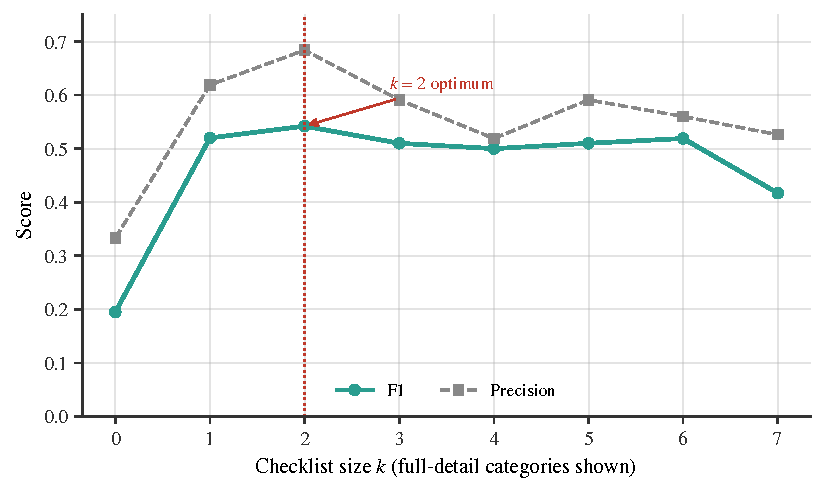
\includegraphics[width=0.7\textwidth]{../images/solana_ksweep.pdf}
    \caption{Solana checklist-size ablation. F1 peaks at $k=2$ and degrades for $k>3$; showing every category in full detail ($k=7$) performs worse than showing none beyond the single best match ($k=1$), confirming that additional retrieved detail dilutes rather than aids the audit once the model's attention budget is exceeded.}
    \label{fig:solana_ksweep}
\end{figure}

F1 peaks at $k=2$ and declines beyond $k=3$; at $k=7$, both precision and recall fall below their $k=1$ values. RAG contributes substantially regardless of $k$ (F1 rises from 0.195 to $\geq$0.500 for every $k$ from 1 to 6), but more checklist detail is not uniformly better: past two or three well-ranked candidates, additional entries appear to dilute the model's attention rather than add usable signal -- the same qualitative conclusion reached for Algorand's fixed $N=3$, now obtained as an explicit measurement rather than an a priori choice. $k=2$ was adopted for all subsequent Solana experiments.

Building on $k=2$, the training corpus was iteratively enriched (Section~\ref{sec:dataset_creation}) and the RAG knowledge base's Denial-of-Service coverage was corrected (Section~\ref{sec:solana_ablation}), while the test set was independently expanded from 59 to 97 contracts (Section~\ref{sec:test_set}). Table~\ref{tab:solana_final} reports the resulting final configuration as a mean $\pm$ std over 5 seeded samples; Table~\ref{tab:solana_percategory} breaks recall down by vulnerability category, averaging TP/FP/FN counts across the same 5 samples.

\begin{table}[!h]
\centering
\caption{Solana final configuration, 97-contract test set, mean $\pm$ std over 5 seeded samples.}
\label{tab:solana_final}
\begin{tabular}{lcccc}
\toprule
\textbf{Configuration} & \textbf{Accuracy} & \textbf{Precision} & \textbf{Recall} & \textbf{F1} \\
\midrule
Fine-tuned, no RAG & 0.581$\pm$0.028 & 0.531$\pm$0.071 & 0.346$\pm$0.035 & 0.419$\pm$0.046 \\
\textbf{Fine-tuned + RAG ($k=2$)} & \textbf{0.666$\pm$0.034} & \textbf{0.677$\pm$0.062} & \textbf{0.496$\pm$0.058} & \textbf{0.572$\pm$0.056} \\
\bottomrule
\end{tabular}
\end{table}

\begin{table}[!h]
\centering
\caption{Solana per-category recall, final configuration, mean TP/FP/FN over 5 seeded samples.}
\label{tab:solana_percategory}
\begin{tabular}{lcccc}
\toprule
\textbf{Category} & \textbf{TP} & \textbf{FP} & \textbf{FN} & \textbf{Recall} \\
\midrule
CPI Reentrancy & 4.0 & 2.8 & 2.0 & 67\% \\
Integer Overflow & 4.0 & 0.2 & 3.0 & 57\% \\
Denial of Service & 3.0 & 2.4 & 3.0 & 50\% \\
Unchecked External Calls & 3.0 & 2.2 & 3.0 & 50\% \\
Missing Key Check & 4.4 & 1.2 & 4.6 & 49\% \\
Type Confusion & 3.4 & 1.2 & 4.6 & 42\% \\
Bump Seed Canonicalization & 2.0 & 1.4 & 4.0 & 33\% \\
\bottomrule
\end{tabular}
\end{table}

\subsection{Solana: Root-Cause Ablation and Failure Diagnosis}
\label{sec:solana_ablation}

Table~\ref{tab:solana_ablation} isolates the contribution of each individual intervention applied over the course of the Solana experiments, holding every other variable fixed within each row pair; two rows are retrieval-accuracy-only ablations rather than end-to-end task measurements, and one is reported as confounded rather than clean, in the interest of not overstating what was actually isolated. Every entry in this table is a single greedy run, taken as a debugging trace at the point each intervention was made; the final row's F1=0.602 therefore differs slightly from the 5-seed mean of 0.572$\pm$0.056 reported for the same configuration in Table~\ref{tab:solana_final}, which reflects proper stochastic sampling applied afterward (Section~\ref{sec:rq5_stability}) and is the number that should be cited as this paper's headline Solana result.

\begin{table}[!h]
\centering
\small
\caption{Solana controlled, single-variable ablations.}
\label{tab:solana_ablation}
\begin{tabular}{p{4.3cm}p{3.6cm}ccc}
\toprule
\textbf{Intervention} & \textbf{Held fixed} & \textbf{Before} & \textbf{After} & $\bm{\Delta}$ \\
\midrule
Parser: verdict-line-only vs.\ whole-block substring match & model, static-checklist architecture, 59-contract test set & F1=0.333 & F1=0.353 & +0.020 \\
Architecture: top-$k$ embedding retrieval vs.\ static checklist & model, fixed parser, 59-contract test set & F1=0.353 & F1=0.510 & +0.157 \\
Checklist size: $k=3 \rightarrow k=2$ & model, parser, 59-contract test set & F1=0.510 & F1=0.542 & +0.032 \\
DoS training example (+1 real pair) & model family, 97-contract test set, $k=2$, knowledge base & F1=0.518 & F1=0.561 & +0.043 \\
DoS knowledge-base coverage (+1 reference entry) & model, 97-contract test set, $k=2$ & F1=0.561 & F1=0.602 & +0.041 \\
KB description rewriting \emph{(retrieval accuracy only)} & model, query set ($n=40$), KB entries & 37.5\% top-1 & 30.0\% top-1 & $-$7.5 pp \\
Embedding model: instructor-xl $\rightarrow$ Qwen3-Embedding-4B & model, 81-contract test set, $k=2$ & F1=0.611 & F1=0.575 & $-$0.036 \\
\bottomrule
\end{tabular}
\end{table}

The first two rows decompose what earlier reporting had recorded only as a single combined jump from F1=0.333 to F1=0.542: re-parsing the \emph{same} static-checklist model outputs with a corrected parser, without touching the retrieval architecture, recovers only F1=0.353 (+0.020); the dominant contribution is reverting the retrieval architecture itself (+0.157), previously conflated with the parser fix because both changes had originally been applied simultaneously. This decomposition required no new GPU inference -- it was obtained entirely by re-parsing already-saved raw model responses.

The two negative-$\Delta$ rows are reported deliberately rather than omitted. Rewriting the knowledge base's per-category descriptions to remove a boilerplate sentence shared across all 37 entries was a reasonable hypothesis -- shared text was suspected to dilute category-specific embedding signal -- but measured worse on an isolated, controlled retrieval test and was reverted before it could affect end-to-end results. Replacing the embedding model with a newer, more discriminative one (cosine-similarity range 0.49--0.86 vs.\ instructor-xl's compressed 0.92--0.98 range in a matched comparison) \emph{did} improve isolated retrieval accuracy, yet \emph{did not} improve downstream, end-to-end F1 when propagated through the identical pipeline on identical model weights and test data -- a direct caution against reporting gains on an intermediate retrieval metric as if they were the result of interest.

Two categories remained comparatively weak even in the final configuration (Table~\ref{tab:solana_percategory}), and inspection of raw model outputs distinguished two qualitatively different causes. For \textbf{Denial of Service}, the model's reasoning trace frequently identified the correct underlying mechanism (e.g., explicitly noting a removed reinitialization guard) but the final verdict named a different category; inspection of the five pre-existing DoS knowledge-base entries showed all five described unrelated sub-patterns (unbounded list growth, unchecked-arithmetic panics, stale price data, missing withdrawal limits), none matching a missing reinitialization guard despite it being the category's own primary textbook example. Adding one targeted reference entry moved this category's retrieval rank from 4th--7th to 1st for three of four previously low-ranking contracts (verified in an isolated retrieval test before the full evaluation) and raised end-to-end recall from 1/6 to 3/6 -- a knowledge-base \emph{coverage} gap, not a retrieval-quality or model-capability gap. For \textbf{Bump Seed Canonicalization}, by contrast, the model's own explanation in several cases correctly and explicitly describes the vulnerable mechanism (e.g., ``uses \texttt{create\_program\_address} with the provided bump'') yet the final verdict is nonetheless ``Not Vulnerable'' -- a \emph{reasoning} failure downstream of correct evidence, which knowledge-base or training-data changes of the kind applied here are unlikely to fix, and which we flag as an open problem in Section~\ref{sec:threats}.

\subsection{Cross-Language Comparison}
\label{sec:cross_language}

Table~\ref{tab:cross_language_comparison} places the two languages' Qwen3-32B measurements -- the one model evaluated on both -- side by side for each of the four experimental configurations, mean $\pm$ std over 5 seeded samples.

\begin{table}[ht]
\centering
\begin{tabular}{ll cccc}
\toprule
\textbf{Experiment} & \textbf{Language} & \textbf{Accuracy} & \textbf{Precision} & \textbf{Recall} & \textbf{F1} \\
\midrule
\multirow{2}{*}{Base, no RAG} & Algorand & 0.315$\pm$0.069 & 0.486$\pm$0.096 & 0.425$\pm$0.071 & 0.453$\pm$0.082 \\
                               & Solana   & 0.423$\pm$0.031 & 0.362$\pm$0.031 & 0.304$\pm$0.035 & 0.330$\pm$0.028 \\
\midrule
\multirow{2}{*}{Base + RAG}   & Algorand & 0.597$\pm$0.047 & 0.742$\pm$0.039 & 0.730$\pm$0.048 & 0.735$\pm$0.038 \\
                               & Solana   & 0.453$\pm$0.025 & 0.387$\pm$0.028 & 0.663$\pm$0.027 & 0.488$\pm$0.027 \\
\midrule
\multirow{2}{*}{Fine-tuned, no RAG} & Algorand & 0.450$\pm$0.049 & 0.613$\pm$0.047 & 0.610$\pm$0.045 & 0.612$\pm$0.046 \\
                                     & Solana   & 0.581$\pm$0.028 & 0.531$\pm$0.071 & 0.346$\pm$0.035 & 0.419$\pm$0.046 \\
\midrule
\multirow{2}{*}{Fine-tuned + RAG}   & Algorand & \textbf{0.675$\pm$0.051} & \textbf{0.792$\pm$0.059} & \textbf{0.805$\pm$0.021} & \textbf{0.798$\pm$0.036} \\
                                     & Solana   & \textbf{0.666$\pm$0.034} & \textbf{0.677$\pm$0.062} & \textbf{0.496$\pm$0.058} & \textbf{0.572$\pm$0.056} \\
\bottomrule
\end{tabular}
\caption{Cross-language comparison of the four experimental configurations, Qwen3-32B, mean $\pm$ std over 5 seeded samples. Algorand figures use the 45-contract test set throughout; for the no-RAG rows the model frequently reports multiple findings per contract, so raw TP+TN+FP+FN can exceed 45 and accuracy is computed as (TP+TN)/(TP+TN+FP+FN) over these totals, consistent with the RAG rows. Solana figures use the 97-contract expanded test set throughout.}
\label{tab:cross_language_comparison}
\end{table}

\begin{figure}[!h]
    \centering
    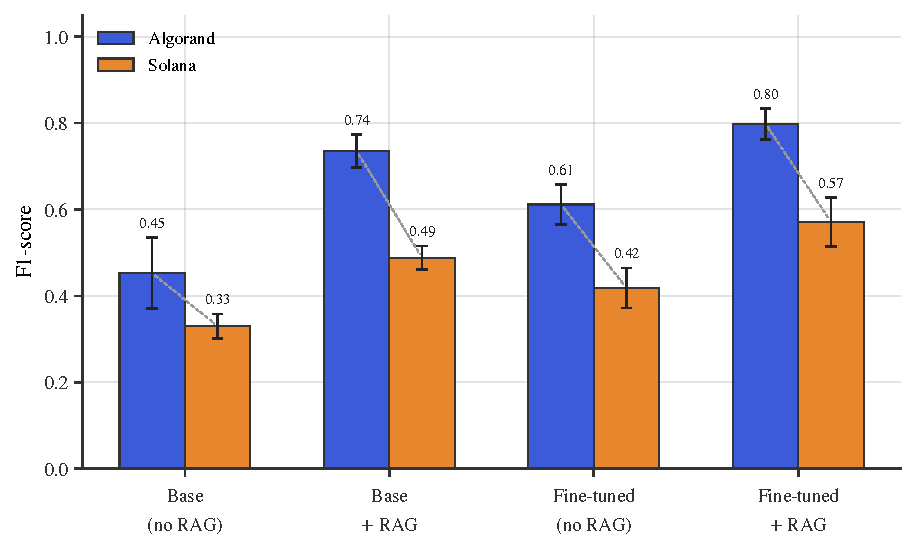
\includegraphics[width=0.75\textwidth]{../images/cross_language_comparison.pdf}
    \caption{Cross-language comparison of all four configurations (F1-score), mean $\pm$ std over 5 seeded samples. The ordering Base $<$ Base+RAG $<$ FT $<$ FT+RAG holds identically in both languages -- the qualitative conclusion generalizes -- while every Solana bar sits below its Algorand counterpart, reflecting the added cross-instruction and cross-program-invocation reasoning burden of the Solana taxonomy (Section~\ref{sec:sealevel}).}
    \label{fig:cross_language_bars}
\end{figure}

Two conclusions hold across both languages, and one difference is stark. First, the \emph{qualitative pattern} of Section~\ref{sec:rag_impact_analysis} replicates exactly: RAG improves mean F1 over the corresponding no-RAG configuration for both the base and the fine-tuned model, and fine-tuning improves mean F1 over the corresponding base configuration both without and with RAG, so the best result in both languages is fine-tuning combined with RAG. Second, the two components' \emph{relative} contributions also track: RAG's absolute F1 gain is larger for the base model than for the fine-tuned model in both languages (Algorand: +0.282 vs.\ +0.186; Solana: +0.158 vs.\ +0.153), consistent with retrieval compensating more for missing task-specific knowledge than for already-imperfect reasoning that fine-tuning has not fully corrected.

The stark difference is absolute performance: every Solana configuration trails its Algorand counterpart, by 0.12--0.25 mean F1 points depending on configuration (largest at Base+RAG, smallest at Base no-RAG). We attribute this gap primarily to task structure rather than to any single fixable defect in the Solana pipeline. PyTeal's transaction-level checks are largely local -- a single field on a single transaction either is or is not validated -- whereas the Solana vulnerability classes studied here (Missing Key Check, Type Confusion, CPI Reentrancy, Unchecked External Calls, Bump Seed Canonicalization) routinely require tracing an account or value across multiple instructions and, in the CPI cases, across a program boundary, which is a substantially higher-entropy reasoning task in the sense of Section~\ref{sec:model_selection}. This is consistent with the Bump Seed Canonicalization finding of Section~\ref{sec:solana_ablation}, where the model's own stated reasoning is frequently correct but the final aggregation into a verdict is not -- exactly the failure mode one would expect from a cross-instruction reasoning task pushed to the edge of a 32B model's reliable range, rather than from a knowledge or retrieval deficit. A secondary contributor is training-data volume: the Solana CoT corpus (267 pairs) is roughly half the size of the Algorand corpus ($\sim$500 instances), and unlike Algorand, no QwQ (reasoning-specialized) variant or SOTA-generalist comparison had been run for Solana at the time of this table, so we cannot yet attribute the residual gap between the two languages' ceilings to model choice versus task difficulty versus data volume with the same confidence achieved for the within-language ablations of Sections~\ref{sec:impact_finetuning} and~\ref{sec:solana_ablation}.

\subsection{Stability Under Repeated Stochastic Sampling}
\label{sec:rq5_stability}

Every result reported in Sections~\ref{sec:impact_finetuning}--\ref{sec:cross_language} is a mean over $N=5$ independently seeded samples per configuration, rather than a single run, for a specific reason: an earlier version of the evaluation harness passed \texttt{temperature=0.6, top\_p=0.95} to \texttt{model.generate()} \emph{without} setting \texttt{do\_sample=True}, which in the \texttt{transformers} version used here silently disables sampling, so every previously "sampled" result in this line of work had in fact been a single deterministic greedy decode with no measured variance. We treat the correction of this bug, and the resampling it required, as itself a finding worth reporting: the point estimates it exposed as unreliable directly motivated two further, independent bug discoveries described below.

\subsubsection{Sampling variance}

Table~\ref{tab:stability_full} reports the standard deviation of F1-score, over 5 seeded samples, for every Algorand and Solana configuration in this study. Standard deviations range from 0.014 (QwQ-32B-FT + RAG, Algorand, our most stable configuration) to 0.082 (Qwen3-32B base, no RAG, Algorand), and are, for several configurations, large enough that a single unlucky or fortunate seed could shift a reported F1 by more than the gain attributed to an intervention such as RAG or fine-tuning alone -- the reason we report every headline number in this paper as mean $\pm$ std rather than as a point estimate.

\begin{table}[!h]
\centering
\small
\caption{F1-score stability over 5 seeded samples, all configurations evaluated in this study.}
\label{tab:stability_full}
\begin{tabular}{llcc}
\toprule
\textbf{Language} & \textbf{Configuration} & \textbf{F1 (mean)} & \textbf{Std} \\
\midrule
\multirow{8}{*}{Algorand} & Qwen3-32B base, no RAG & 0.453 & 0.082 \\
 & Qwen3-32B base + RAG & 0.735 & 0.038 \\
 & Qwen3-32B FT, no RAG & 0.612 & 0.046 \\
 & Qwen3-32B FT + RAG & 0.798 & 0.036 \\
 & QwQ-32B base, no RAG & 0.426 & 0.045 \\
 & QwQ-32B base + RAG & 0.784 & 0.021 \\
 & QwQ-32B FT, no RAG & 0.631 & 0.077 \\
 & QwQ-32B FT + RAG & \textbf{0.814} & \textbf{0.014} \\
\midrule
\multirow{4}{*}{Solana} & Qwen3-32B base, no RAG & 0.330 & 0.028 \\
 & Qwen3-32B base + RAG & 0.488 & 0.027 \\
 & Qwen3-32B FT, no RAG & 0.419 & 0.046 \\
 & Qwen3-32B FT + RAG ($k=2$) & 0.572 & 0.056 \\
\bottomrule
\end{tabular}
\end{table}

Two patterns hold across both languages. First, \textbf{RAG reduces variance as well as raising the mean}: for 7 of the 8 base-vs.-RAG or FT-vs.-RAG pairs, the RAG condition has a lower or equal standard deviation than the corresponding no-RAG condition, consistent with retrieved context anchoring the model's reasoning to concrete, on-demand evidence rather than to a more variable free recall of parametric knowledge. Second, \textbf{the best configuration is also the most stable}: QwQ-32B-FT + RAG achieves both the highest mean F1 on Algorand (0.814) and the lowest variance (0.014) of any configuration in the study, indicating that its advantage over other configurations is not an artifact of favorable seeds.

\subsubsection{Bugs surfaced by scrutinizing implausible numbers}

Refusing to accept an early resampled result at face value -- an initial Algorand base, no-RAG run under the corrected \texttt{do\_sample=True} setting returned near-zero F1, implausibly low relative to the same model's already-published greedy-decode performance -- led to root-causing two further, independent defects, neither of which is specific to sampling.

First, the base (non-fine-tuned) Algorand model's system-level instructions had been sent under a \texttt{"developer"} chat-template role, inherited unchanged from an earlier notebook; a direct \texttt{apply\_chat\_template} test showed this role is silently dropped by the Qwen3/QwQ chat template, so the base model received no formatting instructions at all in no-RAG mode and produced free-form text with no parseable verdict -- a total format collapse masked, for the \emph{fine-tuned} model, by its having internalized the \texttt{<think>}/\texttt{<final>} format during training regardless of prompt content. Switching the role to \texttt{"system"} (confirmed, via the same direct test, to survive the chat template for both models) resolved this.

Second, the no-RAG system prompt asked the model to report its verdict under the header \texttt{"\#\#\# Vulnerability name (if any):"}, while the automated parser's regular expression matched only the exact string \texttt{"\#\#\# Vulnerability:"} on the same or next line; because the regular expression does not match across newlines, this mismatch caused it to capture only the leftover word "name:" rather than the vulnerability name the model had in fact stated on the following line, depressing recall for reasons unrelated to model capability. Rewriting the prompt to use the parser's exact expected phrasing resolved this. Both fixes were applied uniformly across all Algorand no-RAG configurations before the results in Table~\ref{tab:stability_full} were generated; neither defect affected the RAG-mode prompts, which had already used correct phrasing, nor any Solana configuration, which used a different, already-compatible prompt template throughout.

This scrutiny is why every number in Sections~\ref{sec:impact_finetuning}--\ref{sec:cross_language} reflects the corrected pipeline rather than the single greedy run an earlier version of this study relied on.

\subsection{Computational Overhead of RAG}
Retrieval augmentation is not free: embedding the query and performing vector search adds roughly 200--500\,ms of latency per contract, and injecting retrieved snippets and checklists increases prompt length by an estimated 40--60\%, proportionally increasing prefill time and, for API-billed models, inference cost. In a security-audit context, however, this overhead is negligible relative to the cost of a missed exploitable vulnerability, and we consider the trade-off strongly favorable given the observed reduction in false negatives.

\subsection{Summary}
\label{sec:results_summary}

Returning to the two research questions posed in Section~\ref{sec:intro}, in light of both languages and the corrected, resampled pipeline:

\rqanswer{RQ1}{RAG alone is \emph{not} sufficient to close the domain gap for medium-scale (32B) models on either language: fine-tuned + RAG outperforms base + RAG by 0.063 mean F1 on Algorand (Qwen3-32B: 0.798$\pm$0.036 vs.\ 0.735$\pm$0.038) and by 0.084 on Solana (0.572$\pm$0.056 vs.\ 0.488$\pm$0.027; Table~\ref{tab:cross_language_comparison}), and QwQ-32B shows the same pattern on Algorand (0.814$\pm$0.014 vs.\ 0.784$\pm$0.021). For the SOTA generalist DeepSeek-V3.2, by contrast, in-context retrieval alone lifts F1 from 0.767 to 0.94 (Table~\ref{tab:rag_comparison_full}) without any weight update -- a larger absolute gain than RAG achieves for either 32B model, and sufficient on its own to reach near-ceiling performance. Fine-tuning therefore remains necessary to make the most of retrieval at 32B scale in both languages tested, even though, on its own and without RAG, it is no longer sufficient to match a much larger generalist (Section~\ref{sec:benchmark_deepseek}).}

\rqanswer{RQ2}{The answer to RQ1 is scale-dependent, and this dependence is not an artifact of a single language. A $>$600B-parameter generalist converts retrieval into near-optimal accuracy directly and without fine-tuning; medium-scale open models require fine-tuning to extract a comparable, though smaller, gain from the same retrieved context, on both Algorand and Solana. This qualitative pattern -- and the fact that RAG's absolute F1 gain is consistently larger for base than for fine-tuned models (Algorand: +0.282 vs.\ +0.186; Solana: +0.158 vs.\ +0.153) -- replicates across both languages even though no SOTA-generalist comparison was run on Solana. The absolute performance ceiling itself is not language-independent, however: every Solana configuration trails its Algorand counterpart by 0.12--0.25 F1 (Section~\ref{sec:cross_language}), so RQ1 and RQ2's qualitative answers generalize across these two low-resource languages while the quantitative gains they unlock do not.}

\section{Discussion and Threats to Validity}
\label{sec:threats}

Beyond raw accuracy, the choice between fine-tuning and retrieval carries practical implications that we discuss here alongside an explicit assessment of the study's limitations, as is appropriate given the modest scale of the underlying dataset.

\subsection{Practical Implications: Privacy and On-Premise Deployment}
Even where a generalist SOTA model matches or exceeds a fine-tuned specialist on raw metrics, fine-tuned 32B models retain value along two non-functional axes relevant to enterprise adoption. First, \emph{data sovereignty}: auditing proprietary, pre-deployment financial contracts via a third-party cloud API entails transmitting potentially sensitive intellectual property off-premise, a risk that a locally hosted fine-tuned model avoids entirely. Second, \emph{structural determinism}: fine-tuned models internalize the required output schema (the \texttt{<think>}/\texttt{<final>} structure) more reliably than a generalist model steered by prompting alone, which matters for integration into automated pipelines that parse model output programmatically (Section~\ref{sec:eval_pipeline}).

\subsection{Threats to Validity}

\textbf{Dataset scale and statistical power.} The test set contains 45 contracts (5 per vulnerability class); at this scale, single-digit differences in TP/FP/FN counts translate into large swings in precision/recall/F1. We mitigate this by reporting every open-weight configuration as a mean $\pm$ standard deviation over 5 independently seeded samples (Section~\ref{sec:rq5_stability}), rather than a point estimate, but 5 samples is itself a modest number for estimating a standard deviation, and per-category counts (as few as 4--9 examples per class on both languages) remain small enough that individual misclassifications materially shift reported per-category recall. We did not perform paired significance testing (e.g., McNemar's test) across configurations; doing so, ideally with a larger test corpus, is a priority for follow-up work.

\textbf{Single-run evaluation for the SOTA generalist.} DeepSeek-V3.2, accessed via a metered third-party API, is reported as a single inference pass per contract, at unspecified/default sampling temperature, unlike every open-weight configuration; consequently, its comparisons in Table~\ref{tab:sota_comparison} and Table~\ref{tab:rag_comparison_full} lack the variance estimate available for the other rows, and a difference near the observed open-weight standard deviations should be treated with corresponding caution.

\textbf{Potential pretraining data overlap (contamination).} The training and RAG corpora were sourced from Algorand's official, public PyTeal repository \citep{algorand_pyteal_github}. Because this same repository plausibly appears in the pre-training corpora of the general-purpose models evaluated here (including the "base" Qwen3/QwQ models and DeepSeek-V3.2), we cannot rule out that some templates were seen during pre-training. This is a genuine confound for any claim about a model's "intrinsic" (parametric) capability on unseen PyTeal code, and should be treated as a caveat on the base-model results in Section~\ref{sec:impact_finetuning} in particular; a decontamination check (e.g., $n$-gram overlap between the pre-training-adjacent public corpus and our evaluation contracts) is not currently reported and is recommended before drawing strong conclusions about zero-shot capability gaps.

\textbf{Synthetic vulnerability injection.} Vulnerable variants were produced by manually weakening checks in otherwise safe templates rather than sourced from a corpus of real-world, in-the-wild exploited contracts. This controls for confounding business-logic variation but may make injected flaws more locally isolated, and therefore more tractable, than vulnerabilities embedded in more convoluted real-world logic; external validity to production Algorand contracts with more complex control flow remains to be established.

\textbf{Automatic, tag-based grading.} Ground-truth comparison relies on regex extraction of a \texttt{<final>} block and string-level matching against a fixed vulnerability vocabulary (Section~\ref{sec:eval_pipeline}); this is efficient at scale but is a coarser signal than expert human review of the full reasoning trace, and cannot detect a technically correct verdict phrased outside the expected vocabulary except through the retry mechanism.

\textbf{Retrieval corpus--query domain match.} The RAG knowledge base and the evaluation contracts both derive from the same source distribution (PyTeal templates from the official Algorand repository and manually injected variants thereof); performance under RAG has not been evaluated against out-of-distribution contract styles (e.g., contracts from a different organization's internal codebase, or written in a idiosyncratic coding style), where semantic-description retrieval (Section~\ref{sec:sec_code_desc}) may be less reliable.

\textbf{Single comparator for the SOTA baseline.} The generalist comparison relies on one model family (DeepSeek-V3.2) accessed via API at one point in time; API-served models are subject to silent version updates, and reproducing the exact reported numbers at a later date is not guaranteed. We report the model version explicitly for this reason, and recommend that replications pin an explicit API snapshot where the provider supports one.

We regard none of these threats as invalidating the qualitative trends reported in Section~\ref{sec:results} -- which are large in magnitude and consistent across two independent model families -- but they bound the precision with which the reported point estimates should be interpreted, and motivate the larger-scale, contamination-controlled replication we outline in Section~\ref{sec:conclusion}.

\subsection{Limitations}
Independent of the validity threats above, the proposed architecture has three structural limitations. First, RAG effectiveness is bounded by knowledge-base coverage: for a genuine zero-day pattern absent from the vector store, the system loses its factual anchor and falls back on parametric knowledge alone. Second, retrieval based exclusively on natural-language descriptions inherits any imprecision, omission, or ambiguity in the LLM-generated description itself, which can misdirect retrieval toward irrelevant context. Third, the current pipeline analyzes each contract in isolation and does not trace state or authority flows across multiple interdependent contracts, so cross-contract vulnerabilities fall outside its current scope.

\section{Conclusion and Future Work}
\label{sec:conclusion}

This paper presented a hybrid, LLM-centric pipeline for vulnerability detection in low-resource smart-contract languages that combines Chain-of-Thought supervised fine-tuning with a semantic-abstraction Retrieval-Augmented Generation module, evaluated it against a state-of-the-art generalist LLM on a held-out Algorand/PyTeal benchmark spanning eight vulnerability classes, and independently replicated the core pipeline on a second, structurally different language, Solana/Rust, spanning seven classes, with every open-weight result reported as a mean $\pm$ standard deviation over 5 seeded samples rather than a point estimate.

The central empirical finding is that the necessity of fine-tuning is scale-dependent, and that this dependence generalizes across both languages tested. For a massive generalist model (DeepSeek-V3.2), benchmarked on Algorand, in-context retrieval alone was sufficient to reach near-ceiling performance (F1 = 0.94, recall = 0.97, single run) without any weight update, suggesting that for sufficiently large pre-trained models, engineering the retrieval context is a more efficient investment than fine-tuning. For medium-scale, locally deployable models (32B parameters), fine-tuning remained necessary to convert the same retrieved context into comparable gains, though it does not fully close the gap to the generalist: our best on-premise Algorand configuration, QwQ-32B fine-tuned and augmented with RAG, reached F1 = 0.814$\pm$0.014, roughly 13 points below the single-run SOTA generalist while remaining deployable under full data sovereignty; the same recipe applied to Solana with Qwen3-32B reached F1 = 0.572$\pm$0.056, following the identical qualitative pattern at a lower absolute ceiling attributable primarily to Solana's added cross-instruction reasoning burden (Section~\ref{sec:cross_language}). Considered independently, fine-tuning's dominant effect was a reduction in hallucinated false positives (e.g., a mean 18.2$\rightarrow$15.4 FP on Qwen3-32B, Algorand, no RAG), while RAG's dominant effect was a joint improvement in precision and recall across every tested configuration in both languages, confirming its role as a grounding mechanism against statistical over-generalization; RAG also reduced sample-to-sample variance in most configurations, an effect only visible once repeated stochastic sampling was introduced (Section~\ref{sec:rq5_stability}).

These findings refine the picture from our earlier study \citep{boi2025}: fine-tuning is not a universal prerequisite for auditing these languages, but rather a targeted remedy for a specific, practically important scenario -- organizations restricted to on-premise, medium-scale open models for data-sovereignty or cost reasons -- that narrows, without eliminating, the gap to a much larger generalist model once combined with RAG.

Future work should address the threats to validity identified in Section~\ref{sec:threats} through a larger, decontamination-audited benchmark with repeated-sampling variance estimates and paired significance testing. Architecturally, we see three directions. First, moving from the current static, single-pass retrieval pipeline to an \emph{agentic workflow} in which the model can iteratively invoke tools -- static analyzers to offload mechanical checks, the native PyTeal/TEAL compiler to validate hypotheses in real time, and the RAG index itself as a callable tool queried adaptively based on partial findings -- rather than receiving a fixed context bundle upfront. Second, extending retrieval beyond natural-language descriptions toward a \emph{hybrid semantic-structural} representation, indexing generalized function signatures or statement-level abstractions (with identifiers removed) alongside the current text description, in the spirit of Vul-RAG \citep{vulrag2024} and PropertyGPT \citep{propertygpt2025}, to reduce the description-quality bottleneck identified in Section~\ref{sec:threats}. Third, extending the analysis scope from single-contract to \emph{cross-contract} reasoning, tracing global-state and authority flows across interdependent Algorand applications, which the current architecture does not support.

\section*{CRediT authorship contribution statement}
\textbf{Nicola Tortora:} Methodology, Software, Data curation, Investigation, Writing -- original draft. \textbf{Biagio Boi:} Conceptualization, Methodology, Supervision, Writing -- review \& editing. \textbf{Christiancarmine Esposito:} Supervision, Writing -- review \& editing.

\section*{Declaration of competing interest}
The authors declare that they have no known competing financial interests or personal relationships that could have appeared to influence the work reported in this paper.

\section*{Data availability}
Code, prompts, the fine-tuning dataset, and model configurations are publicly available at \url{https://github.com/NickTor99/llm_based_vulnerability_detection_algorand}.

\section*{Acknowledgments}
%% Insert funding/acknowledgment statement here if applicable.

\bibliographystyle{elsarticle-num}
\bibliography{refs}

\end{document}
